% Options for packages loaded elsewhere
\PassOptionsToPackage{unicode}{hyperref}
\PassOptionsToPackage{hyphens}{url}
%
\documentclass[
]{book}
\usepackage{amsmath,amssymb}
\usepackage{lmodern}
\usepackage{ifxetex,ifluatex}
\ifnum 0\ifxetex 1\fi\ifluatex 1\fi=0 % if pdftex
  \usepackage[T1]{fontenc}
  \usepackage[utf8]{inputenc}
  \usepackage{textcomp} % provide euro and other symbols
\else % if luatex or xetex
  \usepackage{unicode-math}
  \defaultfontfeatures{Scale=MatchLowercase}
  \defaultfontfeatures[\rmfamily]{Ligatures=TeX,Scale=1}
\fi
% Use upquote if available, for straight quotes in verbatim environments
\IfFileExists{upquote.sty}{\usepackage{upquote}}{}
\IfFileExists{microtype.sty}{% use microtype if available
  \usepackage[]{microtype}
  \UseMicrotypeSet[protrusion]{basicmath} % disable protrusion for tt fonts
}{}
\makeatletter
\@ifundefined{KOMAClassName}{% if non-KOMA class
  \IfFileExists{parskip.sty}{%
    \usepackage{parskip}
  }{% else
    \setlength{\parindent}{0pt}
    \setlength{\parskip}{6pt plus 2pt minus 1pt}}
}{% if KOMA class
  \KOMAoptions{parskip=half}}
\makeatother
\usepackage{xcolor}
\IfFileExists{xurl.sty}{\usepackage{xurl}}{} % add URL line breaks if available
\IfFileExists{bookmark.sty}{\usepackage{bookmark}}{\usepackage{hyperref}}
\hypersetup{
  pdftitle={Méthodes quantitatives},
  pdfauthor={Paul Hobeika},
  hidelinks,
  pdfcreator={LaTeX via pandoc}}
\urlstyle{same} % disable monospaced font for URLs
\usepackage{color}
\usepackage{fancyvrb}
\newcommand{\VerbBar}{|}
\newcommand{\VERB}{\Verb[commandchars=\\\{\}]}
\DefineVerbatimEnvironment{Highlighting}{Verbatim}{commandchars=\\\{\}}
% Add ',fontsize=\small' for more characters per line
\usepackage{framed}
\definecolor{shadecolor}{RGB}{248,248,248}
\newenvironment{Shaded}{\begin{snugshade}}{\end{snugshade}}
\newcommand{\AlertTok}[1]{\textcolor[rgb]{0.94,0.16,0.16}{#1}}
\newcommand{\AnnotationTok}[1]{\textcolor[rgb]{0.56,0.35,0.01}{\textbf{\textit{#1}}}}
\newcommand{\AttributeTok}[1]{\textcolor[rgb]{0.77,0.63,0.00}{#1}}
\newcommand{\BaseNTok}[1]{\textcolor[rgb]{0.00,0.00,0.81}{#1}}
\newcommand{\BuiltInTok}[1]{#1}
\newcommand{\CharTok}[1]{\textcolor[rgb]{0.31,0.60,0.02}{#1}}
\newcommand{\CommentTok}[1]{\textcolor[rgb]{0.56,0.35,0.01}{\textit{#1}}}
\newcommand{\CommentVarTok}[1]{\textcolor[rgb]{0.56,0.35,0.01}{\textbf{\textit{#1}}}}
\newcommand{\ConstantTok}[1]{\textcolor[rgb]{0.00,0.00,0.00}{#1}}
\newcommand{\ControlFlowTok}[1]{\textcolor[rgb]{0.13,0.29,0.53}{\textbf{#1}}}
\newcommand{\DataTypeTok}[1]{\textcolor[rgb]{0.13,0.29,0.53}{#1}}
\newcommand{\DecValTok}[1]{\textcolor[rgb]{0.00,0.00,0.81}{#1}}
\newcommand{\DocumentationTok}[1]{\textcolor[rgb]{0.56,0.35,0.01}{\textbf{\textit{#1}}}}
\newcommand{\ErrorTok}[1]{\textcolor[rgb]{0.64,0.00,0.00}{\textbf{#1}}}
\newcommand{\ExtensionTok}[1]{#1}
\newcommand{\FloatTok}[1]{\textcolor[rgb]{0.00,0.00,0.81}{#1}}
\newcommand{\FunctionTok}[1]{\textcolor[rgb]{0.00,0.00,0.00}{#1}}
\newcommand{\ImportTok}[1]{#1}
\newcommand{\InformationTok}[1]{\textcolor[rgb]{0.56,0.35,0.01}{\textbf{\textit{#1}}}}
\newcommand{\KeywordTok}[1]{\textcolor[rgb]{0.13,0.29,0.53}{\textbf{#1}}}
\newcommand{\NormalTok}[1]{#1}
\newcommand{\OperatorTok}[1]{\textcolor[rgb]{0.81,0.36,0.00}{\textbf{#1}}}
\newcommand{\OtherTok}[1]{\textcolor[rgb]{0.56,0.35,0.01}{#1}}
\newcommand{\PreprocessorTok}[1]{\textcolor[rgb]{0.56,0.35,0.01}{\textit{#1}}}
\newcommand{\RegionMarkerTok}[1]{#1}
\newcommand{\SpecialCharTok}[1]{\textcolor[rgb]{0.00,0.00,0.00}{#1}}
\newcommand{\SpecialStringTok}[1]{\textcolor[rgb]{0.31,0.60,0.02}{#1}}
\newcommand{\StringTok}[1]{\textcolor[rgb]{0.31,0.60,0.02}{#1}}
\newcommand{\VariableTok}[1]{\textcolor[rgb]{0.00,0.00,0.00}{#1}}
\newcommand{\VerbatimStringTok}[1]{\textcolor[rgb]{0.31,0.60,0.02}{#1}}
\newcommand{\WarningTok}[1]{\textcolor[rgb]{0.56,0.35,0.01}{\textbf{\textit{#1}}}}
\usepackage{longtable,booktabs,array}
\usepackage{calc} % for calculating minipage widths
% Correct order of tables after \paragraph or \subparagraph
\usepackage{etoolbox}
\makeatletter
\patchcmd\longtable{\par}{\if@noskipsec\mbox{}\fi\par}{}{}
\makeatother
% Allow footnotes in longtable head/foot
\IfFileExists{footnotehyper.sty}{\usepackage{footnotehyper}}{\usepackage{footnote}}
\makesavenoteenv{longtable}
\usepackage{graphicx}
\makeatletter
\def\maxwidth{\ifdim\Gin@nat@width>\linewidth\linewidth\else\Gin@nat@width\fi}
\def\maxheight{\ifdim\Gin@nat@height>\textheight\textheight\else\Gin@nat@height\fi}
\makeatother
% Scale images if necessary, so that they will not overflow the page
% margins by default, and it is still possible to overwrite the defaults
% using explicit options in \includegraphics[width, height, ...]{}
\setkeys{Gin}{width=\maxwidth,height=\maxheight,keepaspectratio}
% Set default figure placement to htbp
\makeatletter
\def\fps@figure{htbp}
\makeatother
\setlength{\emergencystretch}{3em} % prevent overfull lines
\providecommand{\tightlist}{%
  \setlength{\itemsep}{0pt}\setlength{\parskip}{0pt}}
\setcounter{secnumdepth}{5}
\usepackage{booktabs}
\usepackage{booktabs}
\usepackage{longtable}
\usepackage{array}
\usepackage{multirow}
\usepackage{wrapfig}
\usepackage{float}
\usepackage{colortbl}
\usepackage{pdflscape}
\usepackage{tabu}
\usepackage{threeparttable}
\usepackage{threeparttablex}
\usepackage[normalem]{ulem}
\usepackage{makecell}
\usepackage{xcolor}
\ifluatex
  \usepackage{selnolig}  % disable illegal ligatures
\fi
\usepackage[]{natbib}
\bibliographystyle{plainnat}

\title{Méthodes quantitatives}
\author{Paul Hobeika}
\date{2022-02-25}

\begin{document}
\maketitle

{
\setcounter{tocdepth}{1}
\tableofcontents
}
\hypertarget{uxe0-propos-de-ce-document}{%
\chapter*{À propos de ce document}\label{uxe0-propos-de-ce-document}}
\addcontentsline{toc}{chapter}{À propos de ce document}

Cette page accueille les notes de cours de méthodes quantitatives du M1 de Science Po Strasbourg pour l'année 2021-2022. Il s'agit d'une introduction aux statistiques destinée à des étudiant·es de master de sociologie politique. Elle ne requiert pas de bagage préalable en statistique ou en mathématique. Il a été généré par l'extension \href{https://bookdown.org/}{bookdown} de Yihui Xie, et le code source est disponible sur \href{https://github.com/phobeika/quanti}{GitHub}.

\hypertarget{donnuxe9es-et-vocabulaire-de-la-statistique}{%
\chapter{Données et vocabulaire de la statistique}\label{donnuxe9es-et-vocabulaire-de-la-statistique}}

\hypertarget{les-sources-statistiques-en-sociologie}{%
\section{Les sources statistiques en sociologie}\label{les-sources-statistiques-en-sociologie}}

Nous avons évoqué la semaine dernière l'importance de la connaissance des sources statistiques pour la production de savoirs quantitatifs en sciences sociale. Il en existe différents types, qu'il est important de savoir identifier.

\hypertarget{les-enquuxeates-par-questionnaire-produites-par-les-chercheur-es}{%
\subsection{Les enquêtes par questionnaire produites par les chercheur-es}\label{les-enquuxeates-par-questionnaire-produites-par-les-chercheur-es}}

C'est par exemple le cas des données exploitées dans \emph{La distinction} \citep{bourdieu1979} dont nous avons parlé au premier semestre. A partir d'une problématique de départ parfois abstraite (dans le sens pas directement quantifiable), l'élaboration d'un questionnaire a souvent pour objectif de trouver des éléments empiriques concrets qui permettent de rendre opérationnelles certaines notions ou concepts. Par exemple, dans \emph{La distinction}, le questionnaire porte sur les pratiques culturelles et permet d'opérationaliser empiriquement la notion de \emph{capital culturel}.

\begin{quote}
Remarque : si vous souhaitez produire vous-même des données dans le cadre de votre TER et de la validation du cours c'est tout à fait possible, mais nous n'aborderons pas la méthodologie du questionnaire dans ce cours. De bons manuels sont toutefois disponibles, je vous recommande par exemple celui de \citet{bugeja-bloch2021}, chapitres 3 et 4.
\end{quote}

\hypertarget{les-autres-source-de-premiuxe8re-main}{%
\subsection{Les autres source de ``première main''}\label{les-autres-source-de-premiuxe8re-main}}

En réalité, les chercheur-es peuvent effectuer des traitement quantitatifs sur d'autres types de sources que les données issues d'un questionnaire. Pour cette raison, Fanny Bugeja-Bloch et Marie-Paule Couto font une distinction entre les \textbf{techniques d'enquête} et les \textbf{techniques d'analyse} des données.

\begin{figure}
\centering
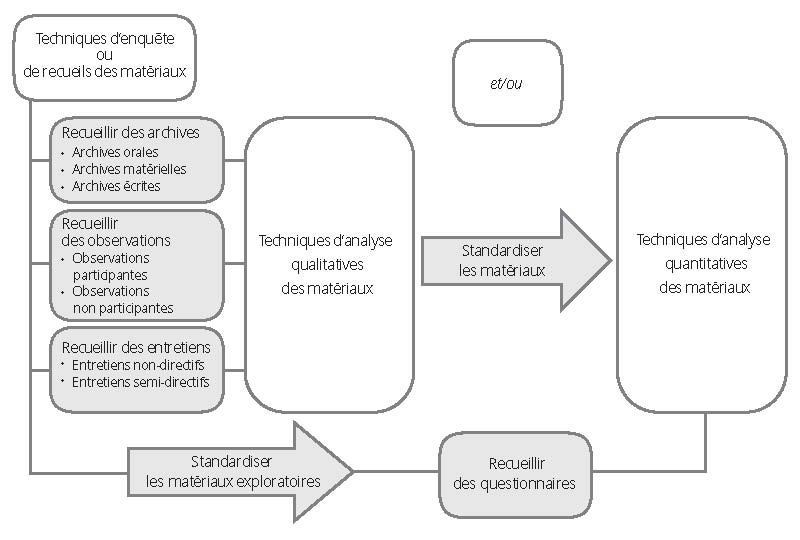
\includegraphics{images/techniquesenquete.jpg}
\caption{Techniques d'enquête et techniques d'analyse \citep{bugeja-bloch2021}}
\end{figure}

Les \textbf{techniques d'enquête} désignent les différents modes de recueil des données : données d'archives, d'entretien ou encore issues d'observation. Les matériaux ainsi produits peuvent ensuite se prêter à différentes formes d'analyse. C'est seulement à ce niveau que l'on peut distinguer méthodes qualitatives et quantitatives. Une analyse qui se fondera sur le commentaire d'un ou quelques extrait d'entretien par exemple sera qualifiée de \emph{qualitative}. Mais ces mêmes matériaux, lorsqu'ils sont \emph{standardisés} et \emph{mis en série} peuvent également être l'objet de techniques d'analyse quantitative. On peut produire des statistiques à partir d'archives \citep{lemercier2008}, à partir d'entretiens (le questionnaire en est un cas particulier) ou encore à partir d'observations \footnote{Un exemple tiré de la sociologie du travail est celui de l'enquête de Jean Peneff sur les urgences. Effectuant une enquête par observation participante en tant que brancardier dans un service d'urgence, il fait un certain nombre de comptages dans l'objectif d'objectiver certaines dimensions du travail aux urgences \citep{peneff1992}.}.

\hypertarget{lanalyse-secondaire-des-donnuxe9es}{%
\subsection{L'analyse secondaire des données}\label{lanalyse-secondaire-des-donnuxe9es}}

Dans de nombreux cas, ce ne sont pas les sociologues ou politistes qui produisent les données qu'ils ou elles exploitent. On parle alors d'\textbf{analyse secondaire des données}. C'est le cas lorsqu'on travaille sur des données de l'Insee ou n'importe quelle base de donnée produite par une administration.

Quelques liens pour accéder aux données de la statistique publique française :

\begin{itemize}
\item
  \href{http://www.progedo-adisp.fr/}{le site de l'Adisp} (Archives de données issues de la statistique publique) , qui rassemble les données de l'Insee et des directions statistiques ministérielles (santé, travail, culture, etc.)
\item
  \href{http://nesstar.ined.fr/webview/}{les données de l'Ined (Institut national de la recherche démographique)}
\end{itemize}

\hypertarget{donnuxe9es-denquuxeate-et-donnuxe9es-de-gestion}{%
\subsection{Données d'enquête et données de gestion}\label{donnuxe9es-denquuxeate-et-donnuxe9es-de-gestion}}

Parmi l'ensemble des données accessibles produites par la statistique publique, on distingue en général deux grandes catégories \citep{desrosières2005} . D'un côté les bases de données produites via une \textbf{enquête par questionnaire} comme évoqué plus haut : elles sont réalisées à partir d'un échantillonage au sein d'une population plus large (voir plus loin pour des définitions de ces termes), et comportent un grand nombre de variables, qui correspondent en général à des questions qui sont posées directement par des enquêteurs ou enquêtrices. De l'autre côté, certaines bases de données sont le \textbf{résultat du travail de gestion de certaines administrations} : par exemple, les employeurs effectuent chaque année ce qu'on appelle une ``déclaration annuelle de données sociales'', dans laquelle ils renseignent une série d'informations sur leurs différents salarié·es (parmi lesquelles leur salaire et leur profession). Ces ``DADS'' constituent un exemple de base de données administrative. Ils sont largement utilisés pour étudier les salaires. Ces bases de données sont intéressantes mais en général moins riches que les données d'enquête, car elles ne sont pas réalisées dans le but de produire de la connaissance. Je vous conseille d'éviter de choisir une telle base de données pour votre rendu du semestre, car il est souvent plus difficile d'en tirer des résultats intéressants à moins de savoir exactement ce qu'on cherche.

\hypertarget{le-vocabulaire-de-la-statistique}{%
\section{Le vocabulaire de la statistique}\label{le-vocabulaire-de-la-statistique}}

\hypertarget{bases-de-donnuxe9es}{%
\subsection{Bases de données}\label{bases-de-donnuxe9es}}

Il est temps d'expliquer plus précisément ce qu'on entend par ``base de données''. En voilà un premier exemple, issu du package R \href{https://cran.r-project.org/web/packages/titanic/titanic.pdf}{\texttt{titanic}} :

\begin{table}

\caption{\label{tab:titanic}Extrait de la base de données des passagers du Titanic}
\centering
\resizebox{\linewidth}{!}{
\begin{tabular}[t]{r|r|r|l}
\hline
PassengerId & Survived & Age & Name\\
\hline
1 & 0 & 22 & Braund, Mr. Owen Harris\\
\hline
2 & 1 & 38 & Cumings, Mrs. John Bradley (Florence Briggs Thayer)\\
\hline
3 & 1 & 26 & Heikkinen, Miss. Laina\\
\hline
4 & 1 & 35 & Futrelle, Mrs. Jacques Heath (Lily May Peel)\\
\hline
5 & 0 & 35 & Allen, Mr. William Henry\\
\hline
6 & 0 & NA & Moran, Mr. James\\
\hline
\end{tabular}}
\end{table}

Une \textbf{base de données} se présente sous la forme d'un tableau. Les lignes décrivent les \textbf{individus} : ici ce sont des passagers, mais gardez en tête que la nature des individus peut être à peu près n'importe quoi (ça peut être des ménages, des villes, des bactéries, n'importe quoi). Chaque colonne apporte des éléments permettant de caractériser les individus (leur nom, leur âge, etc.). On appelle ces caractéristiques des \textbf{variables}.

\hypertarget{un-autre-exemple}{%
\subsection{Un autre exemple}\label{un-autre-exemple}}

Dans cet exemple, les individus sont des États des États-Unis. Les variables correspondent à des taux d'arrestation par la police pour meurtre, agression et viol pour 10000 habitants en 1973, ainsi que le pourcentage de la population urbaine.

\begin{table}

\caption{\label{tab:unnamed-chunk-2}Extrait de la base USArrests}
\centering
\begin{tabular}[t]{l|r|r|r|r}
\hline
  & Murder & Assault & UrbanPop & Rape\\
\hline
Alabama & 13.2 & 236 & 58 & 21.2\\
\hline
Alaska & 10.0 & 263 & 48 & 44.5\\
\hline
Arizona & 8.1 & 294 & 80 & 31.0\\
\hline
Arkansas & 8.8 & 190 & 50 & 19.5\\
\hline
California & 9.0 & 276 & 91 & 40.6\\
\hline
Colorado & 7.9 & 204 & 78 & 38.7\\
\hline
\end{tabular}
\end{table}

\hypertarget{donnuxe9es-tidy}{%
\subsection{Données ``tidy''}\label{donnuxe9es-tidy}}

Dans R, on qualifie certaines base de données de ``tidy'' \citep{wickham2014}. C'est la structure qu'on souhaite avoir en général. Ces bases de données ont un individu par ligne, une variable par colonne. Dans chaque case, on trouve la modalité d'une variable correspondant à l'individu décrit dans la ligne L'exemple présenté sur la figure \ref{fig:tidy} en bas à droite n'est pas ``tidy'', car il existe une variable (dont on ne connaît pas le nom) dont les modalités sont réparties dans deux colonnes différentes, qui représenteny les années 1999 et 2000, c'est-à-dire les modalités d'une autre variable qui indique l'année. En replaçant l'année et la variable observée chacune dans une colonne, on obtient un tableau `tidy' (en bas à gauche).

\begin{figure}
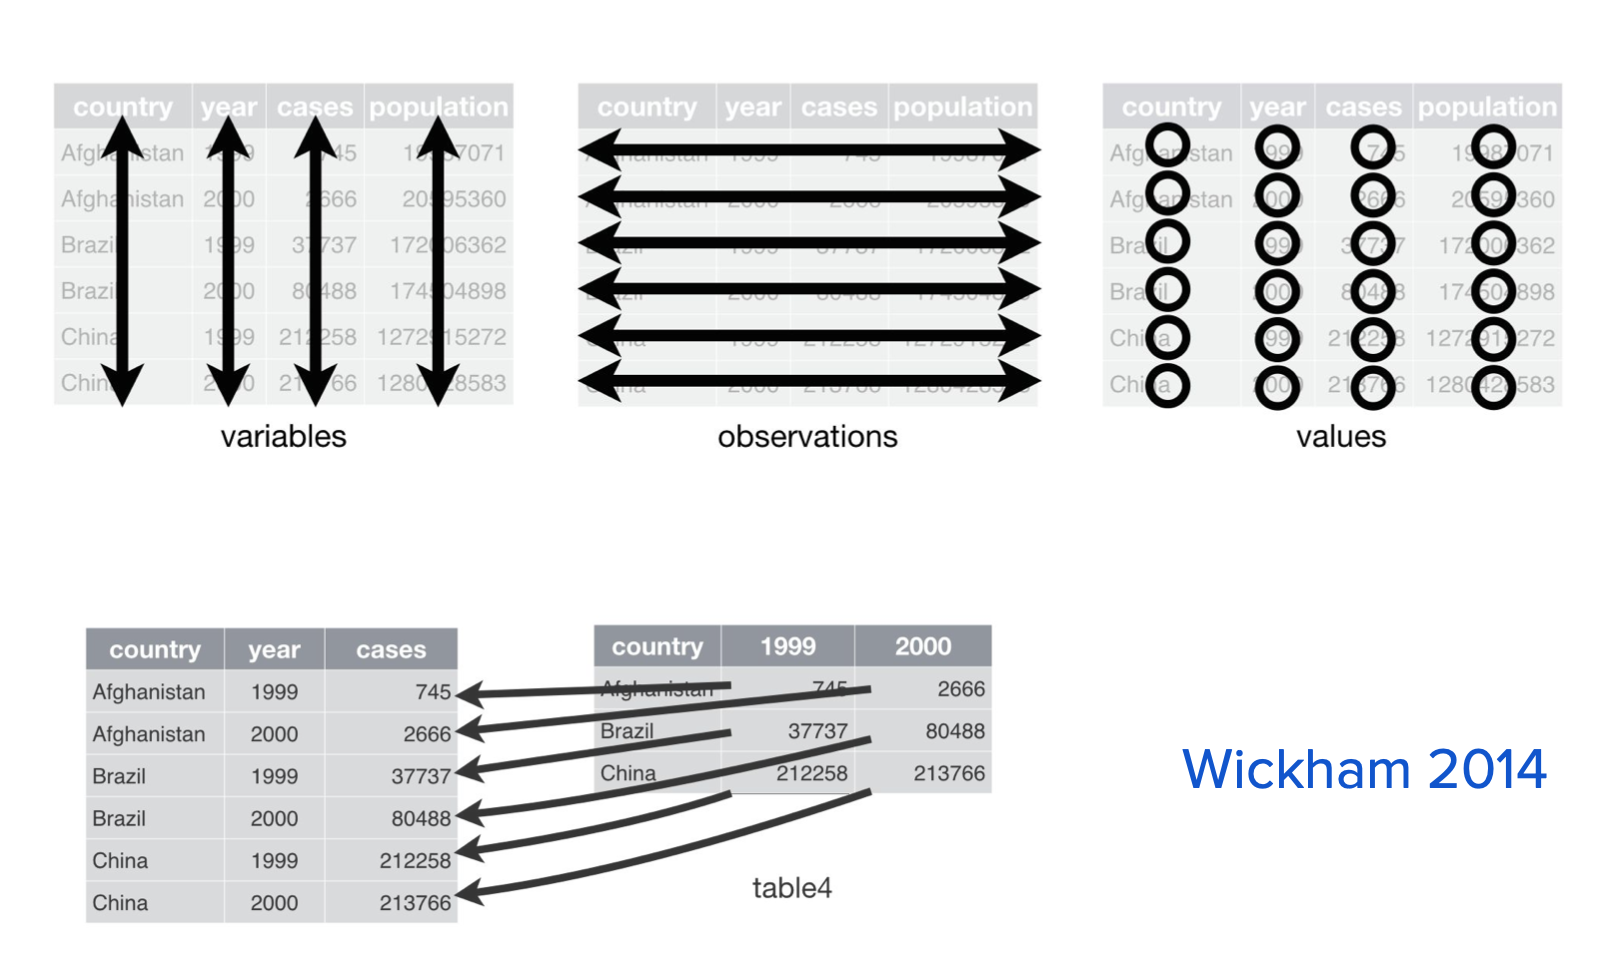
\includegraphics[width=22.36in]{docs/images/tidy} \caption{Tidy data sets}\label{fig:tidy}
\end{figure}

\hypertarget{suxe9ries-temporelles}{%
\subsection{Séries temporelles}\label{suxe9ries-temporelles}}

On parle parfois de \textbf{série temporelle} lorsque une base de donnée concerne un même individu statistique à différents instants. On parle dans ce cas là plutôt d'\textbf{observations} que d'individus. En voilà un exemple : la base de données \texttt{beaver1} accessible dans R présentent la température corporelle d'un castor en fonction du temps.

\begin{table}

\caption{\label{tab:unnamed-chunk-3}Extrait de la base de données beaver1}
\centering
\begin{tabular}[t]{r|r|r|r}
\hline
day & time & temp & activ\\
\hline
346 & 840 & 36.33 & 0\\
\hline
346 & 850 & 36.34 & 0\\
\hline
346 & 900 & 36.35 & 0\\
\hline
346 & 910 & 36.42 & 0\\
\hline
346 & 920 & 36.55 & 0\\
\hline
346 & 930 & 36.69 & 0\\
\hline
\end{tabular}
\end{table}

\hypertarget{autres-types-de-bases-de-donnuxe9es}{%
\subsection{Autres types de bases de données}\label{autres-types-de-bases-de-donnuxe9es}}

\begin{itemize}
\tightlist
\item
  Des données qui décrivent différents individus à un moment donné sont parfois qualifiéed de \textbf{données en coupe} (ou \emph{cross-sectional dataset}). Les données du titanic ou de USArrest en sont des exemples.
\item
  Certaines bases de données décrivent un même groupe d'individus statistique de manière répétée dans le temps. On nomme ce genre de données des \textbf{données de panel} (exemple : enquête Emploi en continu).
\end{itemize}

\hypertarget{variables}{%
\section{Variables}\label{variables}}

\hypertarget{duxe9finition}{%
\subsection{Définition}\label{duxe9finition}}

Les variables sont les éléments qui permettent de décrire les individus présents dans le base de données. Lorsque les données sont issues d'un questionnaire, chaque question correspond en général à une variable.

Exemple :

\begin{itemize}
\tightlist
\item
  le sexe
\item
  la catégorie socioprofessionnelle
\item
  le niveau de diplôme
\item
  le revenu
\end{itemize}

On appelle \textbf{modalités} les différentes valeurs que peuvent prendre une variable.

\begin{figure}
\centering
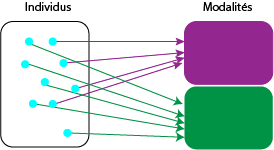
\includegraphics{images/modalites.png}
\caption{Les variables associent les individus à leur modalités}
\end{figure}

\hypertarget{variables-qualitatives-et-variables-quantitatives}{%
\subsection{Variables qualitatives et variables quantitatives}\label{variables-qualitatives-et-variables-quantitatives}}

On distingue les variables en fonction des opérations statistiques qu'on peut effectuer à partir de leurs modalités. Les deux grandes catégories de variables sont les \textbf{variables quantitatives}, dont les modalités sont des nombres, et les \textbf{variables qualitatives}, qui sont les autres.

\hypertarget{variables-qualitatives}{%
\subsection{Variables qualitatives}\label{variables-qualitatives}}

Parmi les variables qualitatives, on distingue encore :

\begin{itemize}
\tightlist
\item
  Les variables \textbf{qualitatives ordinales}, qui sont celles pour lesquelles ont peut ordonner les modalités (exemple : niveau de diplôme)
\item
  Les variables \textbf{qualitatives nominales} dont les modalités ne sont pas hiérarchisables (exemple : sexe, catégorie socioprofesionnelle)
\end{itemize}

\hypertarget{variables-quantitatives}{%
\subsection{Variables quantitatives}\label{variables-quantitatives}}

Les modalités des variables quantitatives (ou numériques) sont des nombres qui ont une signification (par exemple, le code postal n'est pas une variable quantitative). Parmi elles, on distingue :

\begin{itemize}
\tightlist
\item
  Les variables \textbf{continues}, qui peuvent prendre toutes les valeurs réelles dans un intervalle donné
\item
  Les variables \textbf{discrètes}, qui ne peuvent prendre qu'un certain nombre de valeurs
\end{itemize}

\textbf{Pourquoi toutes ces catégories ?} À ces différents types de variables, on associe différentes méthodes statistiques. Il est donc important de comprendre et mémoriser ces définitions, car lorsque vous souhaiterez étudier une variable, la première chose à faire sera d'identifier son type pour ensuite utiliser les méthodes statistiques appropriées.

\hypertarget{mesures-de-tendance-centrale}{%
\section{Mesures de tendance centrale}\label{mesures-de-tendance-centrale}}

Ce sont des manières de résumer l'information contenue dans une variable. En fonction du type de variable, il existe plusieurs indicateurs.

\begin{itemize}
\tightlist
\item
  La \textbf{moyenne} : lorsqu'on parle de moyenne, on fait généralement référence à la moyenne arithmétique d'un ensemble de valeurs numériques (par opposition à la moyenne géométrique ou harmonique). C'est une mesure très utilisée car elle fournit un premier résumé de la distribution statistique. Elle existe uniquement pour les \textbf{variables quantitatives}.
\end{itemize}

\[ \bar{X} = \frac{1}{N}\sum_{i}^{N}{x_i} \]

\begin{itemize}
\item
  La \textbf{médiane} est la modalité d'une variable qui permet de séparer la population en deux parts égales. C'est-à-dire que 50\% des individus auront une modalité supérieure ou égale à la médiane, et 50\% une modalité inférieure ou égale à la médiane.
\item
  Les \textbf{quantiles} sont une généralisation de la médiane : si vous voulez diviser votre population en groupe de 10\%, vous pouvez utiliser les \textbf{déciles}. On appelle la médiane le \textbf{quantile d'ordre 2}, tandis que les déciles sont les \textbf{quantiles d'ordre 10}. Les quantiles les plus utilisés sont la médiane, les quartiles, les déciles et les centiles.
\item
  Les quantiles n'existent que pour les variables dont les modalités peuvent être hiérarchisées : toutes les variables quantitatives et les variables qualitatives ordinales.
\item
  Le \textbf{mode} indique la modalité la plus fréquente d'une variable. Par exemple, la plupart des passagers du Titanic sont décédés dans le naufrage, donc le mode de la variable ``Survived'' est 0. Le mode existe pour tous les types de variables.
\end{itemize}

\hypertarget{univar}{%
\chapter{Statistique descriptive univariée}\label{univar}}

Le cours précédent était consacré à vous présenter différents types de variables. Celui de cette semaine présente les premiers éléments de \textbf{statistique descriptive univariée}, les outils permettant la description d'une unique variable. Ces outils dépendent de la nature de la variable étudiée.

\hypertarget{variables-qualitatives-1}{%
\section{Variables qualitatives}\label{variables-qualitatives-1}}

\hypertarget{tris-uxe0-plat}{%
\subsection{Tris à plat}\label{tris-uxe0-plat}}

Pour décrire ce genre de variable, le principal traitement statistique est de compter le nombre d'individus correspondant à chaque modalité de la variable. C'est ce qu'on appelle un \textbf{tri à plat} (par opposition aux tris croisés qui font intervenir plusieurs variables). Un exemple issu des données du titanic (voir section \ref{tab:titanic}).

\begin{tabular}{l|r|r}
\hline
  & n & \%\\
\hline
1 & 216 & 24.2\\
\hline
2 & 184 & 20.7\\
\hline
3 & 491 & 55.1\\
\hline
Total & 891 & 100.0\\
\hline
\end{tabular}

À partir d'un tableau comportant une ligne par passager, on produit donc un tableau qui comporte seulement une ligne par classe de passagers. La colonne d'effectif montre le nombre de passagers par classe, tandis que la colonne de pourcentage indique le pourcentage de passagers des différentes classes parmi l'ensemble de passagers du Titanic. On peut lire le tableau de cette manière : parmi les 891 passagers du Titanic, 216 voyageaient en première classe. On calcule le pourcentage de chaque catégorie en divisant l'effectif de chaque catégorie par l'effectif total, puis en multipliant par 100 (\(\frac{216}{891}*100 = 24,2 \%\)).

Dans le cas où la variable est qualitative ordinale (c'est-à-dire qu'on peut ordonner ses modalités de manière hiérarchique, comme c'est le cas pour la variable de classe), on peut présenter dans ce tableau les \textbf{pourcentages cumulés}.

\begin{tabular}{l|r|r|r}
\hline
  & n & \% & \%cum\\
\hline
1 & 216 & 24.2 & 24.2\\
\hline
2 & 184 & 20.7 & 44.9\\
\hline
3 & 491 & 55.1 & 100.0\\
\hline
Total & 891 & 100.0 & 100.0\\
\hline
\end{tabular}

Ici, le chiffre 44,9\% représente le pourcentage des passagers qui voyageaient \textbf{au moins en seconde classe}. Il s'agit simplement de la somme des pourcentages des passagers des première et seconde classe. La ligne suivante indique le pourcentage de passagers qui voyageaient au moins en troisième classe, ce chiffre est donc logiquement égal à 100\%.

\hypertarget{diagrammes-en-barre}{%
\subsection{Diagrammes en barre}\label{diagrammes-en-barre}}

La représentation graphique associée à ce décompte est ce qu'on appelle généralement un \textbf{diagramme en barre} (vous pouvez aussi trouver ``diagramme en bâtons ou diagramme en''tuyaux d'orgue" qui désignent la même chose). Sur ce diagramme, on trace des barres verticales dont les hauteurs sont proportionnelles aux effectifs du tri à plat. Seule la hauteur des barres à une signification, la largeur est totalement arbitraire.

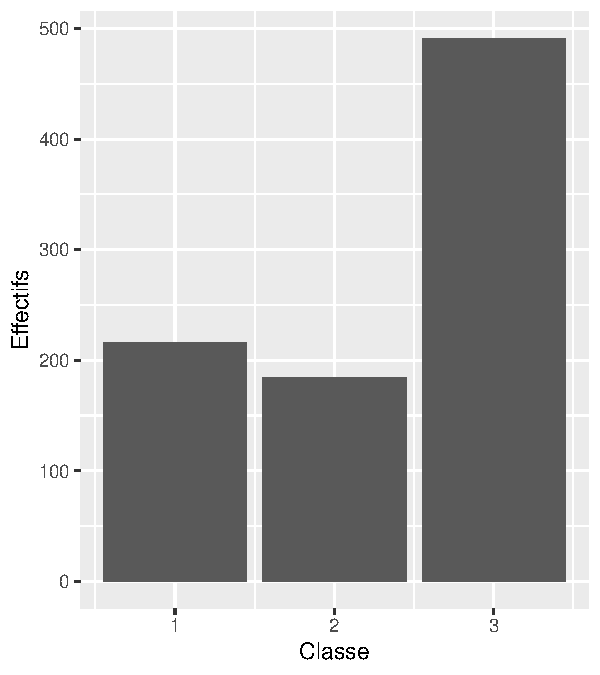
\includegraphics{_main_files/figure-latex/unnamed-chunk-7-1.pdf}

\hypertarget{variables-quantitatives-1}{%
\section{Variables quantitatives}\label{variables-quantitatives-1}}

Si la statistique univariée est très simple pour une variable qualitative, elle peut faire l'objet d'analyses plus approfondies lorsqu'on dispose de variables quantitatives.

\hypertarget{mesures-de-dispersion}{%
\subsection{Mesures de dispersion}\label{mesures-de-dispersion}}

La semaine dernière, je vous ai présenté quelques \textbf{mesures de tendance centrale}. Elles donnent des renseignements importants pour décrire une variable, mais n'en résument qu'une dimension. Deux séries statistiques peuvent avoir la même moyenne tout en étant très différentes.

Comparez par exemple ces deux séries de chiffres, qui représentent des profits (fictifs) en dollars de deux agriculteurs de deux régions A et B :

\begin{itemize}
\tightlist
\item
  A: 14, 16, 18, 20, et 22
\item
  B: 2, 8, 18, 29, et 33
\end{itemize}

La somme de ces deux série est la même, 90 dollars, mais il apparaît rapidement que l'une des séries est beaucoup plus \textbf{dispersée} que l'autre, c'est-à-dire que les écarts par rapport à la moyenne sont en général beaucoup plus grands (la série B). Notre vision des risques et des profits liés à l'agriculture est informée par cette différence, et nous devrions en inclure des indices dans toute description statistique de cette variable.

Pour faire cela, nous avons besoin de mesures permettant de décrire la disperion des modalités de la variable autour de sa moyenne.

\hypertarget{luxe9tendue}{%
\subsubsection{L'étendue}\label{luxe9tendue}}

C'est la différence entre la plus grande et la plus petite valeur de la série :

\[R = X_{max} - X_{min}\]

C'est une mesure de dispersion assez basique. Son défaut est assez évident : elle dépend uniquement des valeurs extrêmes, et aucunement du reste de la distribution.

\hypertarget{luxe9cart-interquartile}{%
\subsubsection{L'écart interquartile}\label{luxe9cart-interquartile}}

Pour prendre en compte plus que les deux valeurs extrêmes, on peut calculer la différence entre deux quantiles, des quartiles par exemple (voir définition dans le premier cours)

\[ Q_d = Q_3 - Q_1 \]

C'est un mesure un peu meilleure que l'étendue, parce que le maximum et le minimum sont des valeurs qui donnent généralement peu d'information sur la distribution en général. Cet écart représente l'étendue de la moitié de la distribution, moitié obtenue après avoir enlevé les 25\% des valeurs les plus faibles et 25\% des valeurs les plus hautes. L'écart interquartile est moins sensible aux valeurs extrêmes que l'étendue (puisqu'on les a supprimées), mais résume tout de même l'ensemble de données sans prendre en compte la variabilité des données entre le premier et le 3ème quartile. Les mesures suivantes n'ont pas ces défauts.

\hypertarget{la-variance}{%
\subsubsection{La variance}\label{la-variance}}

Ce qu'on voudrait, c'est l'équivalent de la moyenne, mais pour mesurer la dispersion. On pourrait donc se dire qu'il suffirait de faire la \textbf{moyenne des écarts à la moyenne} de cette manière \footnote{Les deux côtés de l'équation représentent la même chose, il s'agit juste d'une différence de notation. À gauche, on utilise \ldots{} pour indiquer la série de termes supplémentaires qu'on va inclure dans l'addition mais qu'on n'écrira pas. À droite, l'opérateur \(\sum_{i = 1}^{n}\) est la somme pour i allant de 1 à n de l'expression qui est à droite. Cela signifie qu'il faut remplacer i par 1, puis par 2, 3, etc. jusqu'à n et faire la somme de tous les éléments ainsi obtenu. Ce qui revient exactement à ce qui est écrit de manière plus longue de l'autre côté de l'équation.}:

\[ \frac{1}{N}( (X_1 - X_m) + (X_2 - X_m) + ... + (X_n - X_m) = \frac{1}{n} \sum_{i = 1}^{n} (X_i - X_m) \]

Le problème, en faisant ça, c'est que compte tenu de la définition de la moyenne, les écarts à la moyenne vont se compenser terme à terme. On peut le voir facilement si l'on sépare la somme en deux :

\[ \frac{1}{n} \sum_{i = 1}^{n} (X_i - X_m) = \frac{1}{n} \sum_{i = 1}^{n} X_i - \frac{1}{n} \sum_{i = 1}^{n} X_m \]

Du côté droit de l'équation, le terme de gauche (\(\frac{1}{n} \sum_{i = 1}^{n} X_i\)) est la définition de la moyenne (c'est la somme des termes \(X_1+X_2+...+X_n\) divisé par l'effectif total n), tandis qu'à droite (\(\frac{1}{n} \sum_{i = 1}^{n} X_m\)) on ajoute n fois la moyenne \(X_m\) puis on la divise par n, donc on obtient encore la moyenne. Au final, cette somme est toujours égale à 0.

Pour éviter ce problème, on définit la variance comme la somme des écarts à la moyenne \textbf{au carré}.

\[ Var = \frac{1}{n} \sum_{i = 1}^{n} (X_i - X_m)^2 \]

Cette définition a l'avantage de donner un résultat non nul, excepté dans le cas où la variable est une constante (qui est alors toujours égale à sa moyenne). Surtout, les écarts à la moyenne s'ajoutent, qu'ils soient générés par des valeurs supérieures ou inférieures à la moyenne.

\hypertarget{luxe9cart-type}{%
\subsubsection{L'écart type}\label{luxe9cart-type}}

La variance a beaucoup de propriétés intéressantes et on l'utilise très largement en statistique. Malgré tout, elle a un dernier inconvénient, c'est de s'exprimer comme un carré de l'unité dans laquelle est mesurée la variable. Par exemple, si l'on mesure la taille des étudiant-es de la classe puis qu'on calcule la variance, on aura un résultat en centimètres ou en mètres au carré. Dans notre exemple, on obtient une mesure en ``dollars au carré'', dont le sens est difficile à interpréter.

On résoud ce problème de manière simple en calculant la racine carrée de la variance. Cette opération nous permet d'obtenir notre dernière mesure de dispersion, \textbf{l'écart-type}.

\[ \sigma = \sqrt{\frac{1}{n} \sum_{i = 1}^{n} (X_i - X_m)^2} \]

L'écart-type est la mesure de dispersion la plus utile et la plus fréquente. Elle est meilleure que la variance car elle se mesure dans la même unité que la variable en question. Par exemple, on peut dire que dans la région A, la moyenne des revenus agricoles est de 18 dollars, avec un écart-type de 2,8 dollars.

\hypertarget{repruxe9sentations-graphiques}{%
\subsection{Représentations graphiques}\label{repruxe9sentations-graphiques}}

Il existe plusieurs manières de représenter graphiquement la distribution d'une variable quantitative.

\hypertarget{histogramme}{%
\subsubsection{Histogramme}\label{histogramme}}

Les histogrammes sont l'équivalent des diagrammes en barres pour les variables quantitatives. Chaque barre (ou rectangle) qui compose l'histogramme a une aire qui est proportionnelle au nombre d'observation dont les valeurs sont dans l'intervalle sur lequel s'étend le rectangle.

\begin{figure}
\centering
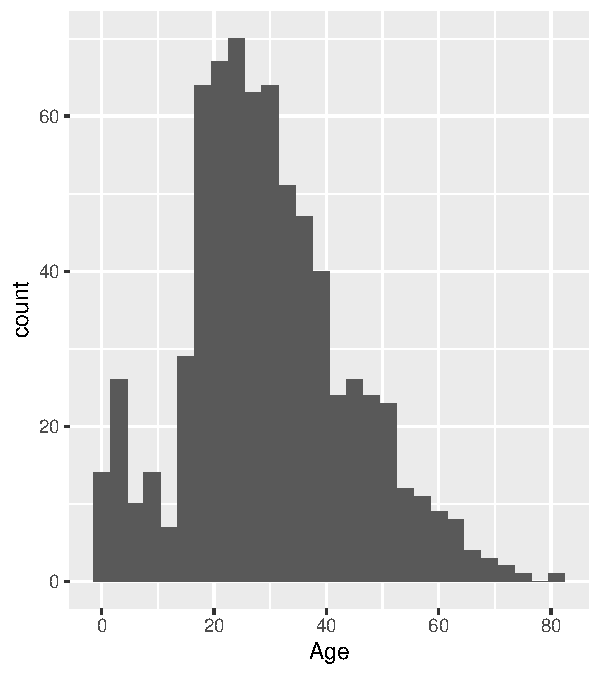
\includegraphics{_main_files/figure-latex/unnamed-chunk-8-1.pdf}
\caption{\label{fig:unnamed-chunk-8}Distribution de l'âge des passagers du Titanic. Chaque rectangle a une largeur de 3 ans}
\end{figure}

Comme il s'agit de variables quantitatives, on peut choisir le nombre de rectangles comme on le souhaite (contrairement aux variables qualitative dont les modalités sont définies une fois pour toutes). Ici, on représente la même variable avec moins de rectangles.

\begin{figure}
\centering
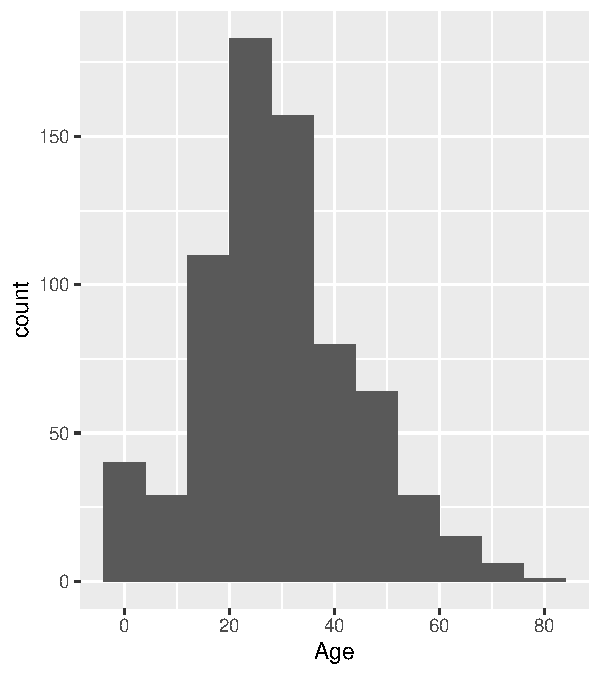
\includegraphics{_main_files/figure-latex/unnamed-chunk-9-1.pdf}
\caption{\label{fig:unnamed-chunk-9}Même figure avec une largeur de 8 ans}
\end{figure}

Ici avec un plus grand nombre de rectangle (largeur = 1 an)

\begin{figure}
\centering
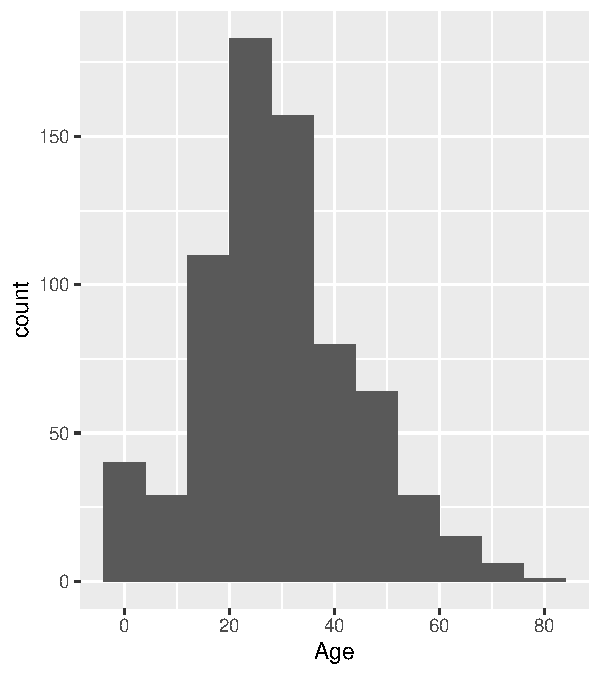
\includegraphics{_main_files/figure-latex/unnamed-chunk-10-1.pdf}
\caption{\label{fig:unnamed-chunk-10}Même figure avec une largeur d'un an}
\end{figure}

\hypertarget{densituxe9}{%
\subsubsection{Densité}\label{densituxe9}}

On représente parfois les variables quantitatives par une courbe que l'on appelle une `densité'. C'est la courbe qu'on pourrait obtenir si on avait un très grand nombre de passagers et qu'on représentait l'histogramme avec des rectangles très fins.

On peut également produire une estimation de cette courbe à partir d'une transformation effectuée sur les histogrammes. Si l'on trace une ligne qui passe au milieu de chacun des segments supérieurs des rectangles qui composent l'histogramme, on obtient alors un graph qu'on nomme un \textbf{polygone de fréquence}.

\begin{figure}
\centering
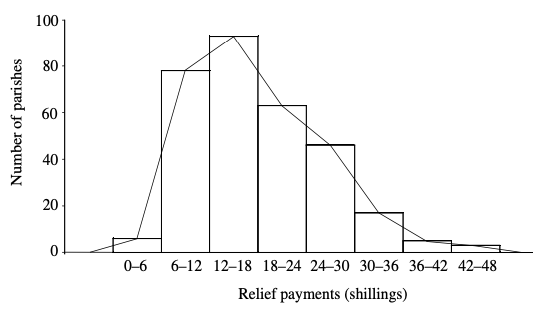
\includegraphics[width=3.125in,height=\textheight]{images/frequencypol.png}
\caption{\emph{Per capita} relief payments in 311 parishes in 1831 (Fenstein \& Thomas, p.~41)}
\end{figure}

La forme de ce polygone peut être être ``lissée'' à l'aide de techniques mathématiques, pour donner la courbe de densité recherchée. Elle donne une idée de la forme du polygone de fréquence si l'on avait un très grand nombre d'individu dans notre échantillon.

\begin{figure}
\centering
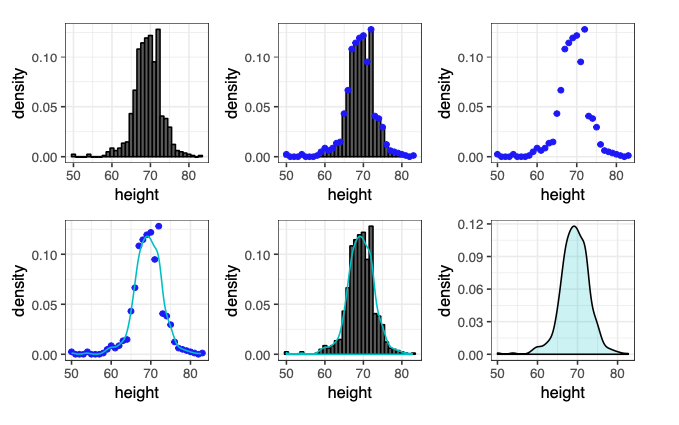
\includegraphics{images/density.png}
\caption{D'un histogramme à une densité de probabilité}
\end{figure}

Ces représentations graphiques sont un bon moyen de visualiser la \textbf{forme} de la distribution d'une variable quantitative continue, et spécifiquement de la manière dont les données sont réparties autour de leur valeur ``centrale''.

\hypertarget{asymuxe9trie-skewness}{%
\subsubsection{\texorpdfstring{Asymétrie (\emph{skewness})}{Asymétrie (skewness)}}\label{asymuxe9trie-skewness}}

Une manière de caractériser les distribution est leur symétrie par rapport à la moyenne. Les valeurs peuvent en effet être réparties de manière symétrique de part et d'autre de la moyenne, ou bien de manière asymétrique (\emph{skewed}).

\begin{figure}
\centering
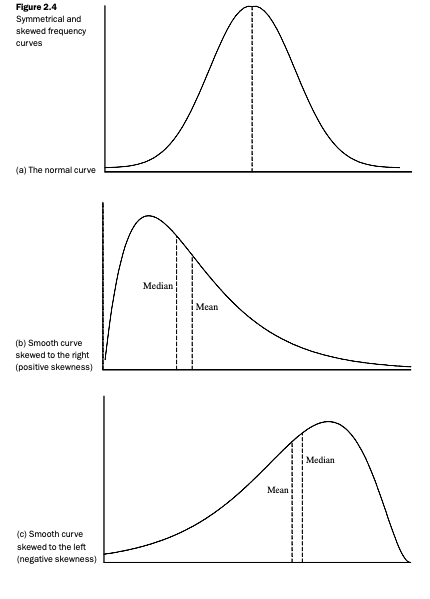
\includegraphics{images/skewed.png}
\caption{Distributions symétriques et asymétriques \citep[p.54]{feinstein2002}}
\end{figure}

Différentes mesures permettent de quantifier l'asymétrie d'une distribution.

\begin{itemize}
\tightlist
\item
  Elles doivent être indépendantes de l'unité de mesure
\item
  Et elle doivent être nulles lorsque la distribution est symétrique.
\end{itemize}

Un exemple de coefficient d'asymétrie est le suivant, mais il en existe d'autres :

\[ Skewness = \frac{3*(Mean - Median)}{\sigma} \]

Un exemple de variable dont la distribution est asymétrique est la distribution des revenus dans la population française. L'histogramme suivant représente la distribution du niveau de vie (c'est le revenu des ménages divisé par le nombre d'\href{https://www.insee.fr/fr/metadonnees/definition/c1890}{unités de consommation}). Le niveau de vie médian (compris dans la portion verte du graphique) est inférieur au niveau de vie moyen, car les ménages au niveaux de vie très élevés (en bleu) tirent la moyenne vers le haut, mais n'ont pas d'effet sur la médiane.

\begin{figure}
\centering
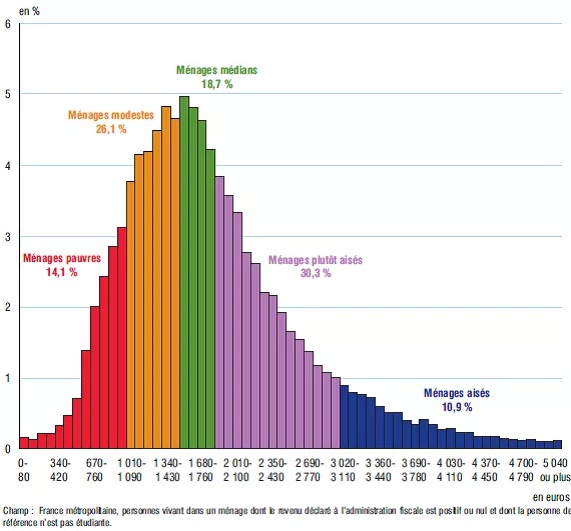
\includegraphics{images/salaires - copie.jpg}
\caption{Distribution des niveaux de vie mensuels en 2014 en France (Source : Insee, Portrait social 2014)}
\end{figure}

\hypertarget{loi-normale}{%
\section{La loi normale : une distribution importante}\label{loi-normale}}

La loi normale est une distribution théorique, définie à partir de son expression mathématique. Mais bien que théorique, c'est une distribution très importante, car elle est souvent utilisée comme approximation de distributions réelles. Je vous la présente ici rapidement, on la retrouvera dans des prochaines séances.

Pour définir une loi normale, il faut connaître deux constantes : sa moyenne \(X_m\) et l'écart type \(\sigma\). L'équation donne la valeur de Y (la hauteur de la courbe, qui apparaît sur l'axe des ordonnées) pour tout valeur de X (mesuré sur l'axe des abscisses) :

\[ Y(X) = \frac{1}{ \sigma \sqrt{2\pi}} exp(- \frac{(X - X_m)^2}{2*\sigma^2})\]

La fonction \(exp()\) qui apparaît dans la formule est la \textbf{fonction exponentielle}. Si vous ne connaissez pas cette fonction, sachez qu'elle est définie par le fait qu'il s'agit de l'unique fonction \(f(x)\) qui est toujours égale à sa dérivée (la fonction dérivée est celle qui mesure la pente de la courbe en chaque point, on la note \(f'(x)\) : elle est positive lorsque \(f\) est croissante, et négative lorsqu'elle est décroissante) et qui est égale à 1 lorsque \(x = 0\). Comme elle est toujours égale à sa dérivée, plus \(x\) est élevé, plus la fonction exponentielle doit avoir une dérivée élevée, donc plus elle doit croître rapidement.

\begin{Shaded}
\begin{Highlighting}[]
\FunctionTok{curve}\NormalTok{(}\FunctionTok{exp}\NormalTok{(x), }\AttributeTok{from=}\SpecialCharTok{{-}}\DecValTok{5}\NormalTok{, }\AttributeTok{to=}\DecValTok{5}\NormalTok{, , }\AttributeTok{xlab=}\StringTok{"x"}\NormalTok{, }\AttributeTok{ylab=}\StringTok{"y"}\NormalTok{)}
\end{Highlighting}
\end{Shaded}

\begin{figure}
\centering
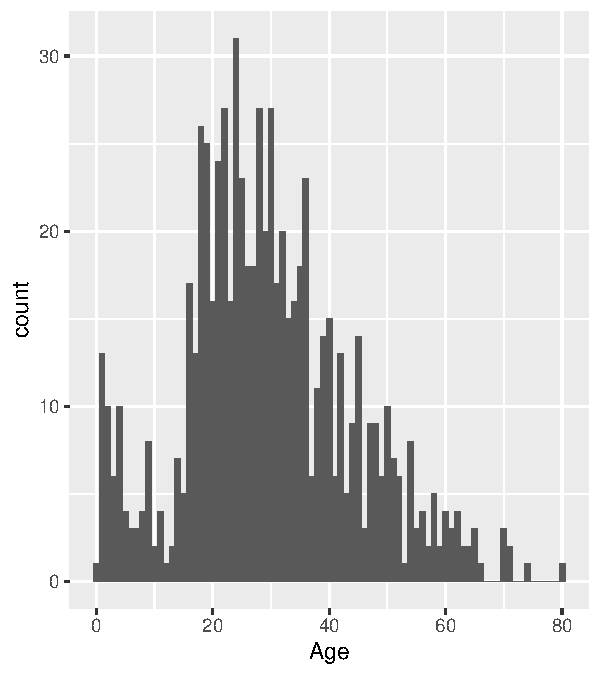
\includegraphics{_main_files/figure-latex/unnamed-chunk-11-1.pdf}
\caption{\label{fig:unnamed-chunk-11}Graphe de la fonction exponentielle entre -5 et 5}
\end{figure}

Dans la distribution de la loi normale, la fonction exponentielle contient une expression qui est toujours inférieure ou égale à zéro. Son maximum est donc atteint lorsque \(X\) est égal à sa moyenne \(X_m\), auquel cas \(Y(X_m) = \frac{1}{ \sigma \sqrt{2\pi}}\). Plus \(X\) va s'éloigner de sa moyenne, plus \(Y(X)\) sera faible, on dit que la distribution \textbf{tend vers 0 lorsque X tend vers ``moins l'infini'' ou ``plus l'infini''}. Le graphe de la loi normale ressemble donc à une sorte de dos d'âne, ce qui explique qu'on l'appelle aussi ``la courbe en cloche''.

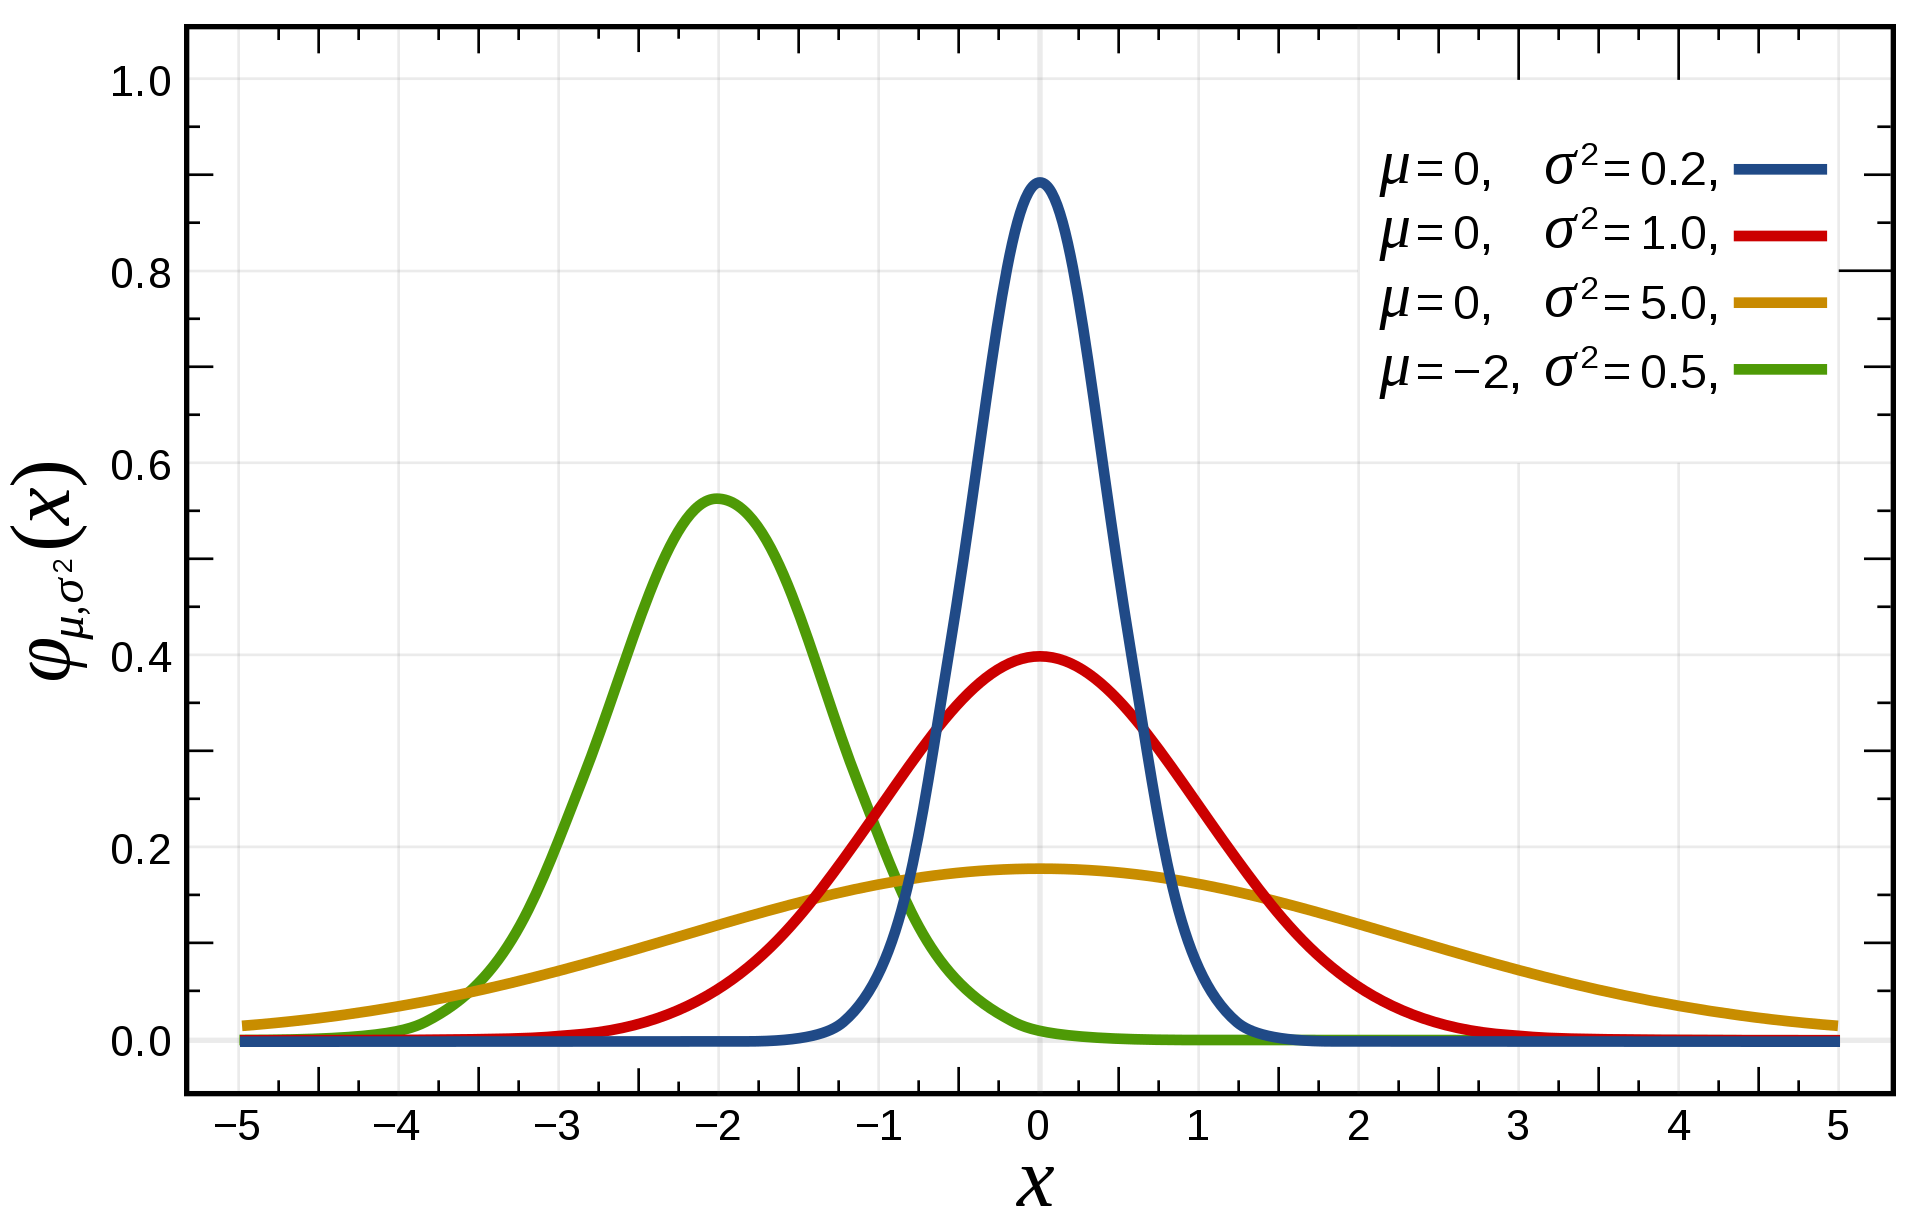
\includegraphics{images/loisnormales.png} Ce dernier graphe permet de constater que, si les lois normales ont toutes la même allure, leur forme dépend de la moyenne et de l'écart-type de la distribution. Comme déjà évoqué, la moyenne indique le maximum de la courbe. L'écart-type détermine lui la ``largeur'' de la bosse, c'est-à-dire à quel point les données s'étalent autour de la moyenne.

Une propriété importante de la loi normale est que, quelque soit sa moyenne et son écart-type, il y a toujours une même proportion d'observations qui seront distribués à une certaine distance de la moyenne (que l'on peut mesurer en calculant l'aire sous la courbe), mesurée en nombre d'écarts-type.

Par exemple :

\begin{itemize}
\tightlist
\item
  \textbf{90\% des observations} sont situés à moins de \textbf{1,645 écarts-type} autour de la moyenne, laissant 5\% de chaque côté.
\item
  \textbf{95\% des observations} sont situés à moins de \textbf{1,96 écarts-type} autour de la moyenne, laissant 2,5\% de chaque côté.
\item
  \textbf{99\% des observations} sont situés à moins de \textbf{2,58 écarts-type} autour de la moyenne, laissant 0,5\% de chaque côté.
\end{itemize}

\begin{figure}
\centering
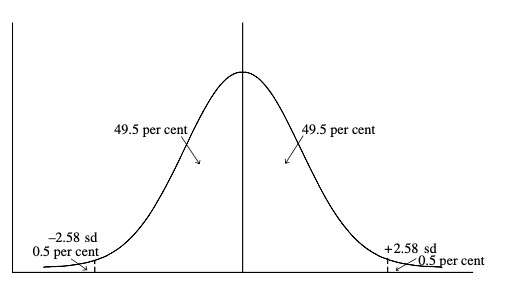
\includegraphics{images/normal.png}
\caption{Aire sous la courbe}
\end{figure}

\hypertarget{cor1}{%
\chapter{Analyse bivariée et corrélation I}\label{cor1}}

Jusque là, on a vu différents outils qui nous permettent de décrire plusieurs types de variables :

\begin{itemize}
\tightlist
\item
  tris à plat (variables qualitatives)
\item
  indices de tendance centrale
\item
  indices de dispersion
\item
  représentations graphiques (diagrammes en barres, histogrammes)
\end{itemize}

C'est-à-dire que ce qu'on sait faire, c'est prendre une variable (par exemple la catégorie socioprofessionnelle d'une personne ou le revenu d'un ménage), et, en fonction du type de variable, en proposer une sorte de résumé, dont la forme dépend de la nature de la variable À partir de maintenant, on va commencer à voir comment étudier les relations entre plusieurs variables. C'est ce qui nous intéresse en général. Le cours de cette semaine ne traite que le cas de \textbf{deux variables qualitatives}.

\hypertarget{les-tableaux-croisuxe9s}{%
\section{Les tableaux croisés}\label{les-tableaux-croisuxe9s}}

Un \textbf{tableau de fréquence} ou \textbf{tableau croisé} est l'outil statistique le plus fréquemment utilisé pour étudier le lien entre deux variables qualitatives. C'est un tableau qui indique la distribution des effectifs d'une population en fonction des modalités de deux variables qualitatives. En voici un premier exemple :

\begin{table}

\caption{\label{tab:unnamed-chunk-14}Répartition des passagers du Titanic par classe et par sexe}
\centering
\begin{tabular}[t]{l|r|r|r|r}
\hline
  & 1 & 2 & 3 & Total\\
\hline
female & 94 & 76 & 144 & 314\\
\hline
male & 122 & 108 & 347 & 577\\
\hline
Total & 216 & 184 & 491 & 891\\
\hline
\end{tabular}
\end{table}

Un tel tableau qui répartit N individus dans 4 cases constitue un système de classification \textbf{exclusif} (chaque individu est dans une seul case) et \textbf{exhaustif} (tous les individus sont dans une case)

\hypertarget{distributions-marginales}{%
\subsection{Distributions marginales}\label{distributions-marginales}}

\begin{table}

\caption{\label{tab:unnamed-chunk-15}Répartition des passagers du Titanic par classe et par sexe}
\centering
\begin{tabular}[t]{l|r|r|r|>{}r}
\hline
  & 1 & 2 & 3 & Total\\
\hline
female & 94 & 76 & 144 & \textcolor{red}{\textbf{314}}\\
\hline
male & 122 & 108 & 347 & \textcolor{red}{\textbf{577}}\\
\hline
\textcolor{red}{\textbf{Total}} & \textcolor{red}{\textbf{216}} & \textcolor{red}{\textbf{184}} & \textcolor{red}{\textbf{491}} & \textcolor{red}{\textbf{\textbf{891}}}\\
\hline
\end{tabular}
\end{table}

La dernière colonne du tableau et la dernière ligne indiquent les totaux pour chaque ligne et colonne. On les appelle les \textbf{distributions marginales}. Un tableau croisé doit toujours comporter ces distributions marginales. Elles correspondent aux tris à plat des deux variable séparées, ici les variables \emph{Sexe} et \emph{Fréquentation du théâtre}.

\hypertarget{distributions-conditionnelles}{%
\subsection{Distributions conditionnelles}\label{distributions-conditionnelles}}

On appelle par contraste les effectifs présents à l'intérieur du tableau les \textbf{distribution conditionnelles}. Chaque case correspond au nombre d'individus concernés simultanément par les deux modalités des deux variables (en ligne et en colonne). Ce tableau est la \emph{distribution de la fréquentation du théâtre en fonction du sexe}.

\begin{table}

\caption{\label{tab:unnamed-chunk-16}Répartition des passagers du Titanic par classe et par sexe}
\centering
\begin{tabular}[t]{l|l|l|l|l}
\hline
  & 1 & 2 & 3 & Total\\
\hline
female & \textcolor{red}{\textbf{94}} & \textcolor{red}{\textbf{76}} & \textcolor{red}{\textbf{144}} & 314\\
\hline
male & \textcolor{red}{\textbf{122}} & \textcolor{red}{\textbf{108}} & \textcolor{red}{\textbf{347}} & 577\\
\hline
Total & 216 & 184 & 491 & 891\\
\hline
\end{tabular}
\end{table}

Le problème avec ce tableau est qu'il est difficile à commenter, car le nombre total de femmes et d'hommes parmi les passagers est différent, et de même le nombre de passagers dans chaque classe est différent. On ne peut donc pas facilement comparer les distributions conditionnelles (le nombre de femmes et d'hommes dans chaque classe). Pour cela, il faut transformer le tableau en utilisant des pourcentages.

Il y a différentes façons de former une table en pourcentages à partir du tableau de fréquence. La première idée serait de calculer les pourcentage de chaque case \textbf{par rapport à l'effectif total}.

\begin{tabular}{l|r|r|r|r}
\hline
  & 1 & 2 & 3 & Total\\
\hline
female & 10.5 & 8.5 & 16.2 & 35.2\\
\hline
male & 13.7 & 12.1 & 38.9 & 64.8\\
\hline
Total & 24.2 & 20.7 & 55.1 & 100.0\\
\hline
\end{tabular}

La transformation effectuée ici consiste à diviser chaque chiffre du tableau par l'effectif total. On obtient ainsi le pourcentage de chaque catégorie parmi l'ensemble des passagers. On peut alors lire les distributions conditionnelles de cette manière : les femmes de 1ère classe représentent 10,5\% de l'ensemble des passagers du Titanic. Les distributions marginales donnent à nouveau les tri à plat des deux variables, exprimés en pourcentages : 35,2\% des passagers sont des femmes, 24,2\% des passagers sont en première classe.

On observe donc que, malgré cette transformation, il est toujours impossible de comparer directement les pourcentages des distributions conditionnelles, car ils sont encore dépendants des distributions marginales. Pour comparer les chiffres présents dans les différentes lignes ou colonnes, il faut se ramener à une situation où le nombre d'hommes ou de femmes serait égal, ou bien le nombre de passagers de chaque classe serait égal.

Pour cela, on calcule des pourcentage \textbf{en ligne} ou des pourcentage \textbf{en colonne}.

\hypertarget{pourcentages-en-ligne-et-en-colonne}{%
\subsection{Pourcentages en ligne et en colonne}\label{pourcentages-en-ligne-et-en-colonne}}

\begin{table}

\caption{\label{tab:unnamed-chunk-18}Pourcentages d'hommes et de femmes parmi chaque classe du Titanic}
\centering
\begin{tabular}[t]{l|r|r|r|r}
\hline
  & 1 & 2 & 3 & Ensemble\\
\hline
female & 43.5 & 41.3 & 29.3 & 35.2\\
\hline
male & 56.5 & 58.7 & 70.7 & 64.8\\
\hline
Total & 100.0 & 100.0 & 100.0 & 100.0\\
\hline
\end{tabular}
\end{table}

Ce tableau est un exemple de pourcentages en colonne Pour l'obtenir, plutôt que calculer des pourcentages par rapport à l'effectif total, on calcule le pourcentage d'hommes et de femmes pour chaque classe, c'est-à-dire qu'on divise les distributions conditionnelles par les effectifs totaux de chaque classe (par exemple, \(94/216*100 = 43,5 \%\) de femmes parmi les passagers de première classe). On se ramène donc à une situation fictive, dans laquelle chaque classe du Titanic aurait 100 passagers et passagères au total, \textbf{mais dont la proportion d'hommes et de femmes parmi chaque classe serait la même que la proportion réelle}.

Se ramener à 100 passagers par classe permet alors de comparer les pourcentages de femmes et d'hommes pour ces différentes classe. Pour commenter le tableau, il faut d'abord lire les pourcentages marginaux : on voit qu'au total il y a 35\% de femmes et 65\% d'hommes parmi les passagers. Ainsi, même si les femmes sont minoritaires en première classe (43,5\%), elles sont surreprésentées par rapport à leur pourcentage parmi l'ensemble des passagers. Elles le sont également en seconde classe, où elles représentent 41,3\% des passagers. Elles sont à l'inverse sous-représentées en troisième classe, où elles sont seulement 29,3\%.

Il est également possible de calculer des pourcentages en ligne.

\begin{table}

\caption{\label{tab:unnamed-chunk-19}Distribution par classe des femmes et des hommes passagers du Titanic}
\centering
\begin{tabular}[t]{l|r|r|r|r}
\hline
  & 1 & 2 & 3 & Total\\
\hline
female & 29.9 & 24.2 & 45.9 & 100\\
\hline
male & 21.1 & 18.7 & 60.1 & 100\\
\hline
Ensemble & 24.2 & 20.7 & 55.1 & 100\\
\hline
\end{tabular}
\end{table}

Ici, on se ramène à une sitaution où il y aurait 100 hommes et 100 femmes sur le bateau, et on compare leur distribution par classe. Ce tableau permet de comparer directement les proportions d'hommes et de femmes parmi les différentes classes. On observe par exemple que la proportion de femmes en première classe (29,9\%) est plus élevée que celle des hommes (21,1\%), et inversement en 3ème classe. On peut encore comparer avec les distributions marginales, mais ici comme il n'y a que deux modalités c'est moins important.

\hypertarget{statistiques-descriptives-et-statistiques-infuxe9rentielles}{%
\section{Statistiques descriptives et statistiques inférentielles}\label{statistiques-descriptives-et-statistiques-infuxe9rentielles}}

Une des caractéristiques des données des passagers du Titanic est qu'elles sont \textbf{exhaustives}, c'est-à-dire que l'on détient des informations pour l'ensemble des passagers. Produire un tableau croisé permet ainsi de pouvoir établir sans ambiguïté les liens entre deux variables qualitatives (par exemple, ici, on peut affirmer que les femmes sont surreprésentées dans les deux premières classes). On parle dans ce cas de \textbf{statistiques descriptives}.

Produire cette affirmation est plus complexe dans le cas où l'on dispose de données produites sur \textbf{un échantillon} d'individus, et que l'on souhaite en déduire des résultats sur une population plus large. C'est cette question qui est au cœur de la \textbf{statistique inférentielle}. Prenons donc un autre exemple, issu des données de l'enquête ``Histoires de vie'' réalisée en 2003 par l'Insee, et dont le package \texttt{questionr} fournit un extrait. On va s'intéresser à la pratique du bricolage.

\begin{table}

\caption{\label{tab:unnamed-chunk-21}Pratique du bricolage par sexe}
\centering
\begin{tabular}[t]{l|r|r|r}
\hline
  & Non & Oui & Total\\
\hline
Homme & 384 & 515 & 899\\
\hline
Femme & 763 & 338 & 1101\\
\hline
Total & 1147 & 853 & 2000\\
\hline
\end{tabular}
\end{table}

On peut de la même manière produire un tableau avec des pourcentages en colonne

\begin{table}

\caption{\label{tab:unnamed-chunk-22}Pratique du bricolage par sexe}
\centering
\begin{tabular}[t]{l|r|r|r}
\hline
  & Non & Oui & Ensemble\\
\hline
Homme & 33.5 & 60.4 & 45\\
\hline
Femme & 66.5 & 39.6 & 55\\
\hline
Total & 100.0 & 100.0 & 100\\
\hline
\end{tabular}
\end{table}

On lit ainsi que, parmi les individus qui font partie de l'échantillon, les hommes sont 60,4\% à déclarer pratiquer le bricolage, contre 39,4\% des femmes. La question est alors de savoir si l'on peut généraliser ce résultat à l'ensemble de la population, c'est-à-dire affirmer que, parmi la population française de plus de 15 ans, les hommes pratiquent plus le bricolage que les femmes.

On conçoit que la réponse à cette question dépend de la manière avec laquelle les individus qui composent l'échantillon ont été sélectionnés. Si les hommes ont été interrogés à la sortie d'un magasin de bricolage, tandis que les femmes ont été sélectionnée d'une autre manière, il est évident que ces résultats ne seront pas généralisable, car l'échantillon ne sera pas \textbf{représentatif} de la population qu'on cherche à décrire.

Pour répondre à cette question, il est donc nécessaire d'avoir un ``bon'' échantillon. On va donc faire comme si l'échantillonnage avait été réalisé de manière \textbf{aléatoire} (ce qui n'est pas forcément vrai pour ce jeu de données qui est seulement un extrait de la base de données `histoire de vie'). Si l'échantillonnage est aléatoire, on peut alors préciser notre question, qui devient : quelle probabilité y a-t-il que les différences observées entre les déclarations des hommes et des femmes interrogées au sujet du bricolage soient l'effet du hasard ? Autrement dit, est-il possible d'expliquer que les hommes soient majoritaires à se déclarer bricoleurs dans notre échantillon par le fait qu'on aurait \emph{par hasard} interrogé des hommes particulièrement bricoleurs, ou des femmes particulièrement peu bricoleuses ?

\hypertarget{le-test-du-chi2}{%
\section{\texorpdfstring{Le test du \(\chi^2\)}{Le test du \textbackslash chi\^{}2}}\label{le-test-du-chi2}}

Pour répondre à cette question, on effectue ce qu'on appelle un \textbf{test d'hypothèse}. Il existe beaucoup de tests différents, mais le test qu'on va utiliser s'appelle le test du \(\chi^2\) (prononcé ki-deux). Il s'agit d'une procédure permettant d'évaluer le \textbf{niveau de significativité d'une relation statistique entre deux variables qualitatives}, ici la relation entre la variable ``Bricolage'' et la variable ``Sexe''.

Les tests d'hypothèse suivent tous la même logique : on commence par faire une hypothèse de départ \textbf{sur la population générale}, et on va ensuite \textbf{tester le caractère plus ou moins plausible de cette hypothèse à partir des données de notre échantillon} (répétons qu'il doit s'agir d'un échantillon aléatoire). Ici, l'hypothèse est que les deux variables ``Sexe'' et ``Bricolage'' ne sont pas corrélées ; on l'appelle \textbf{l'hypothèse nulle}.

\hypertarget{principe-du-test-dhypothuxe8se}{%
\subsection{Principe du test d'hypothèse}\label{principe-du-test-dhypothuxe8se}}

Prenons un exemple plus simple pour bien se représenter le principe. Imaginons qu'on lance une pièce de monnaie pour savoir si elle est équilibrée ou non (c'est-à-dire qu'elle a la même probabilité de tomber sur pile ou face). D'un côté, on fait l'hypothèse qu'elle est équilibrée. De l'autre, on la lance 100 fois, et on observe qu'elle tombe 55 fois sur face et 45 fois sur pile. On chercher à accepter ou à rejeter notre hypothèse de départ à partir de ces chiffres.

On ne peut pas répondre à cette question de manière certaine, mais seulement estimer le \textbf{risque de se tromper}. Accepter ou rejeter l'hypothèse ont chacun leur risque associé :

\begin{itemize}
\tightlist
\item
  le risque d'accepter l'hypothèse alors qu'elle est fausse (par exemple, ici, dire que la pièce est équilibrée)
\item
  le risque de rejeter l'hypothèse alors qu'elle est vraie (ici, dire que la pièce n'est pas équilibrée alors qu'elle l'est)
\end{itemize}

Pour calculer ces deux risques, le principe est toujours de comparer la distribution statistique (ici 45/55) et la distribution théorique à laquelle on s'attendrait si l'hypothèse de départ était vérifiée (ici, 50/50). On appelle ces distributions les \textbf{effectifs observés} et les \textbf{effectifs théoriques}

\hypertarget{effectifs-observuxe9s-et-effectifs-thuxe9oriques}{%
\subsection{Effectifs observés et effectifs théoriques}\label{effectifs-observuxe9s-et-effectifs-thuxe9oriques}}

Si l'on revient à notre exemple, les effectifs observés sont simples à obtenir, il s'agit de notre tableau croisé contenant les effectifs des différentes catégories. Ce sont donc les données déjà présentées :

\begin{table}

\caption{\label{tab:unnamed-chunk-23}Pratique du bricolage par sexe. Effectifs observés.}
\centering
\begin{tabular}[t]{l|r|r|r}
\hline
  & Non & Oui & Total\\
\hline
Homme & 384 & 515 & 899\\
\hline
Femme & 763 & 338 & 1101\\
\hline
Total & 1147 & 853 & 2000\\
\hline
\end{tabular}
\end{table}

Pour savoir quels sont les effectifs théoriques, il faut calculer l'équivalent du ``50/50'' pour la pièce de monnaie, mais dans le cas de notre tableau statistique. La question est donc de savoir, dans le cas où les deux variables ne sont pas corrélées, quels seraient les effectifs d'hommes et de femmes déclarant ou non pratiquer le bricolage.

Répondre à cette question est plus simple qu'il n'y paraît, car si les variables ne sont pas corrélées, la probabilité de pratiquer le bricolage doit être la même pour les hommes et pour les femmes, c'est donc le nombre d'individus déclarant bricoler (853), divisé par l'effectif total (2000). Pour obtenir l'effectif théorique d'hommes bricoleurs, il faut donc multiplier le nombre d'hommes dans notre échantillon (899) par la probabilité d'être bricoleur (853/2000). On obtient de la même façon toute la distribution conditionnelle théorique (remarquez bien qu'on ne change rien aux distributions marginales, elles sont identiques pour les effectifs observés et les effectifs théoriques).

\[ n^{th}_{ij} = \frac{n_i * n_j}{n}\]
où \(n^{th}_{ij}\) est l'effectif théorique de la ligne \(i\) et de la colonne \(j\) (par exemple les hommes bricoleurs), \(n_i\) l'effectif de la colonne \(i\) (les bricoleurs et bricoleuses), \(n_j\) l'effectif de la colonne \(j\) (les hommes), et \(n\) l'effectif total.

\begin{table}

\caption{\label{tab:unnamed-chunk-24}Pratique du bricolage par sexe. Effectifs théorique.}
\centering
\begin{tabular}[t]{l|r|r|r}
\hline
  & Homme & Femme & Total\\
\hline
Non & 515 & 631 & 1147\\
\hline
Oui & 383 & 469 & 853\\
\hline
Total & 899 & 1101 & 2000\\
\hline
\end{tabular}
\end{table}

\hypertarget{calcul-du-chi-2}{%
\subsection{Calcul du chi-2}\label{calcul-du-chi-2}}

Le résultat du test va dépendre de la différence entre les valeurs observées et les valeurs théoriques. Pour estimer ces différences, on calcule ce qu'on appelle le \(\chi^2\) de cette manière :

\begin{enumerate}
\def\labelenumi{\arabic{enumi}.}
\tightlist
\item
  on prend la différence pour chaque case du tableau
\item
  on met ces différences au carré
\item
  on divise le résultat par les fréquences observées
\item
  on fait la somme de ces valeurs
\end{enumerate}

\[\chi_2 = \sum_{ij} \frac{(n^{th}_{ij} - n^{obs}_{ij})^2}{n^{th}_{ij}}\]
Dans notre exemple, le chi-2 serait égal à :

\[ \chi_2 = \frac{(515-384)^2}{515} + \frac{(631-515)^2}{631}+\frac{(383-763)^2}{383} + \frac{(469-338)^2}{469} = 141.93 \]
Mais on aura jamais à le faire à la main, les logiciels le font automatiquement. Une fois cette valeur obtenue, on peut presque répondre à la question. Il nous manque juste un élément : le lien entre cette valeur qui donne une idée de la différence entre les effectifs observés et les effectifs théoriques, et le risque d'erreur que l'on cherchait au début. Là il s'agit d'une question de mathématique qui est au-delà du niveau du cours et qu'il n'est pas nécessaire de maîtriser pour comprendre le principe du test. Admettons donc que nous sommes en mesure de déduire de cette valeur du \(\chi^2\) le risque d'erreur recherché.

Voici ce que nous indique R lorsqu'on lui demande de calculer le \(\chi^2\) pour le tableau présentant le bricolage en fonction du sexe :

\begin{Shaded}
\begin{Highlighting}[]
\FunctionTok{table}\NormalTok{(hdv2003}\SpecialCharTok{$}\NormalTok{sexe, hdv2003}\SpecialCharTok{$}\NormalTok{bricol) }\SpecialCharTok{\%\textgreater{}\%} \FunctionTok{chisq.test}\NormalTok{()}
\end{Highlighting}
\end{Shaded}

\begin{verbatim}
## 
##  Pearson's Chi-squared test with Yates' continuity correction
## 
## data:  .
## X-squared = 141.93, df = 1, p-value < 2.2e-16
\end{verbatim}

R nous affiche d'abord le \(\chi^2\) que nous avons calculé plus haut à la main. \texttt{df} indique le nombre de \textbf{degrés de liberté} du tableau, qui correspond au nombre de colonnes moins 1 multiplié par le nombre de lignes moins 1 (ici \(1*1=1\)). Ce chiffre est nécessaire pour estimer le risque d'erreur (ce qu'on cherche) à partir de la valeur du \(\chi^2\), mais pour nous il n'est pas très important. Il affiche enfin la valeur recherchée, nommée \emph{p-value} : il s'agit du risque de se tromper dans le cas où l'on rejette l'hypothèse nulle, c'est-à-dire l'hypothèse selon laquelle il n'y a pas de lien de corrélation entre les variables. Cette valeur est comprise entre 0 et 1. Pour un même nombre de degrés de liberté, plus la valeur du \(\chi^2\) est élevée, plus ce risque est faible. Ici il est égal à \(2.2e-16\), ce qui signifie \(0,000000000000022 \%\).

Si l'échantillonnage est bien aléatoire, on peut donc affirmer avec confiance qu'au delà de l'échantillon observé, la pratique du jardinage est correlée au sexe des individus. En général, on se fixe un seuil de significativité \emph{a priori} (par exemple 1\%, ou \(\alpha = 0.01\)). Lorsque la \emph{p-value} est inférieure à cette valeur, on va dire qu'on rejette l'hypothèse nulle avec un risque de 1\%, ou encore que \textbf{la corrélation observée est significative au seuil de 1\%}. Attention : si la \emph{p-value} est supérieure à ce seuil, on ne peut pas conclure à la non significativé de la corrélation étudiée. On ne peut simplement pas affirmer avec le seuil de certitude choisi que la corrélation statistique est significative.

Cette méthode permet ainsi d'évaluer le risque d'erreur lorsqu'on cherche à généraliser une corrélation observée sur un échantillon à l'ensemble d'une population. On doit réaliser ce test à chaque fois qu'on veut commenter une relation de corrélation entre deux variables qualitatives, car sinon on risque toujours de commenter en réalité des écarts qui sont liés au hasard de l'échantillonnage. Il faut enfin prendre garde à ne pas faire dire au \(\chi^2\) plus que ce qu'il ne permet d'affirmer. En particulier, le test ne dit rien sur l'intensité de la relation de corrélation, et cela quelle que soit la valeur de la \emph{p-value} obtenue.

\hypertarget{infer}{%
\chapter{Inférence et variables quantitatives}\label{infer}}

Lors du dernier cours, on a abordé certaines notions de statistique inférentielle à partir de l'étude de la corrélation entre deux variables quantitatives. Le cours de cette semaine est consacré à la présentation de l'analyse inférentielle d'une variable quantitative. L'enjeu est de savoir, lorsqu'on réalise des statistiques sur un échantillon, dans quelle mesure il sera possible de généraliser les résultats tels que la moyenne observée d'une variable quantitative. Avant de traiter cette question, je vous présente plus en détail certaines notions de statistique inférentielle déjà abordées, telles que les méthodes d'échantillonnage.

\hypertarget{muxe9thodes-duxe9chantillonage}{%
\section{Méthodes d'échantillonage}\label{muxe9thodes-duxe9chantillonage}}

La statistique inférentielle repose sur la méthode dite des sondages, qui consiste à étudier une population à partir d'un échantillon d'individus sélectionné parmi l'ensemble de cette population.

\begin{figure}
\centering
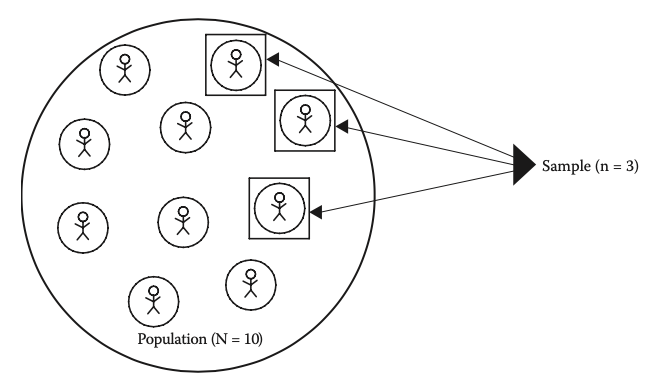
\includegraphics{images/sample.png}
\caption{On utilise souvent des données qui concernent un échantillon pour décrire une population plus large}
\end{figure}

Savoir si oui ou non il est possible de généraliser les résultats obtenus à partir de l'étude d'un échantillon dépend largement de la méthode d'échantillonnage. Il existe en effet des bons et des mauvais échantillons. Contrairement à une croyance longtemps répandue dans la pratique de la statistique, la taille de l'échantillon n'est pas le facteur déterminant de la qualité d'un échantillon. C'est ce qu'a montré George Gallup en 1936, qui a prédit la victoire de Roosevelt aux élections présidentielles états-uniennes à partir d'un échantillon comportant 5000 individus. Dans le même temps, les grands journaux états-uniens prédisaient la victoire de son concurrent à partir de la collecte de plus de deux millions d'intentions de vote. S'il faut bien sur un effectif minimal, il vaut donc mieux avoir un petit échantillon de bonne qualité plutôt qu'un gros échantillon de mauvaise qualité.

Quels sont alors les éléments qui font la qualité d'un échantillon ? Un échantillon est de bonne qualité lorsqu'il a la même structure que la population. On dit alors qu'il est \textbf{représentatif}. On peut dire par exemple que l'échantillon constitué par les lecteurs des quotidiens états-uniens est \textbf{non-représentatif} : les individus de cet échantillon auront des caractéristiques particulières par rapport au reste de la population (par exemple voter plus fréquemment pour le parti républicain). Leurs intentions de vote ne permettent donc pas de prédire les résultats aux élections présidentielles. De la même manière, l'enquête sur les classes sociales menée par l'équipe de sociologues réuni·es autour de Mike Savage au début des années 2010, la \emph{Great british class survey}, a été réalisée par internet en collaboration avec la BBC qui en faisait la promotion à l'aide de spots télévisés. Malgré le succès de l'enquête mesurée en termes du nombre de personnes qui ont participé, l'un des premiers résultats est que les classes populaires sont largement sous représentées dans l'échantillon, et en particulier les fractions les plus précaires \citep{savage2013}.

\hypertarget{les-uxe9chantillons-aluxe9atoires}{%
\subsection{Les échantillons aléatoires}\label{les-uxe9chantillons-aluxe9atoires}}

Il existe en pratique plusieurs méthodes d'échantillonnage qui permettent de produire des échantillons de plus ou moins bonne qualité. La meilleure méthode d'un point de vue statistique est de \textbf{sélectionner l'échantillon de manière aléatoire}.

Une première manière de faire est de réaliser un tirage aléatoire lors duquel tous les individus de la population ont la même probabilité d'être choisis. On parle alors d'\textbf{échantillonnage aléatoire simple}. Cette méthode n'est pas toujours possible à mettre en œuvre car elle implique de disposer d'une liste exhaustive de la population à laquelle on s'intéresse. À partir de ce document qu'on appelle une \emph{base de sondage}, on peut réaliser un tel tirage aléatoire. Dans le cas de la population française, la seule institution à disposer d'une telle liste est l'Insee, ce qui lui confère un forme de monopole sur la production d'échantillons aléatoires, et qui explique que de nombreuses enquêtes produites par l'Ined ou l'Inserm le sont en partenariat avec l'Insee \citep[p.66]{bugeja-bloch2021}.

Dans certains cas, plutôt qu'attribuer une même probabilité de tirage à tous les individus, on souhaite que certaines catégories d'individus soient surreprésentées dans l'échantillon. On parle alors d'\textbf{échantillon aléatoire stratifié}. Un tel échantillon n'est pas représentatif de la population dans son ensemble, mais chaque strate (les différentes catégories d'individus auxquels on a attribué des probabilités différentes d'être sélectionnés) est représentative de la catégorie d'individus qu'elle représente. Par exemple, l'échantillon de l'enquête sur la sexualité des français conduite par l'Ined en 2008 surreprésente volontairement les jeunes, ce qui permet de produire des analyses détaillées de cette sous-population \citep{toulemon2008}.

Enfin, une manière de produire un échantillonnage aléatoire sans disposer d'une base de sondage portant sur les individus est de réaliser ce qu'on appelle un \textbf{échantillonnage par grappe} (ou échantillonnage aréolaire). Cela est possible lorsque les individus sont réunis naturellement en groupes relativement homogènes, et que l'on dispose d'une liste exhaustive de ces groupes, dont la nature peut être variée. Par exemple, l'enquête \textbf{Sans-Domicile 2001} de l'Insee est basée sur un échantillonnage des usagers des services de distributions de repas chaud en hiver. Cet échantillonnage est aréolaire car il repose sur un échantillonnage des villes de plus de 20000 habitants dans lesquels sont localisés ces services, et un autre échantillonnage des distributions de repas eux-mêmes \citep{brousse2005}.

\hypertarget{les-uxe9chantillons-non-aluxe9atoires}{%
\subsection{Les échantillons non aléatoires}\label{les-uxe9chantillons-non-aluxe9atoires}}

Lorsque l'échantillon n'est pas réalisé selon une des méthodes décrite ci-dessus, il n'est pas aléatoire. Les individus n'ont alors pas tous la même probabilité de faire partie de l'échantillon. La méthode non aléatoire la plus utilisée est la méthode dite \textbf{des quotas}, mise en œuvre notamment par les instituts de sondage (IFOP, IPSOS, etc.). Dans ce cas, l'échantillon est constitué à partir d'une définition \emph{a priori} des critères importants de représentativité de la population (sexe, age, catégories socioprofessionnelles par exemple). Il faut donc connaître certaines caractéristiques de la population de référence pour construire un échantillon par quota. L'échantillon ne sera toutefois représentatif que des critères précis sélectionnés en amont, contrairement à un échantillon aléatoire, qui est représentatif quel que soit le critère envisagé (et cela sans avoir à spécifier aucun de ces critères). Un défaut important de ce mode d'échantillonnage est que les individus qui ne souhaitent pas répondre disparaissent de l'échantillon, et il n'est donc pas possible d'en décrire les caractéristiques \citep{lehingue2007}.

Vous pouvez garder en tête que les méthodes de la statistique inférentielle supposent en général que l'on dispose d'un échantillon aléatoire.

\hypertarget{vocabulaire-de-la-statistique-infuxe9rentielle}{%
\section{Vocabulaire de la statistique inférentielle}\label{vocabulaire-de-la-statistique-infuxe9rentielle}}

\hypertarget{paramuxe8tres-et-estimateurs}{%
\subsection{Paramètres et estimateurs}\label{paramuxe8tres-et-estimateurs}}

Revenons maintenant à la question qui nous intéresse. On suppose qu'on dispose d'un échantillon aléatoire et d'une variable quantitative permettant de décrire une caractéristique des individus (par exemple leur taille). On s'intéresse à la différence entre ce que l'on mesure sur cet échantillon (par exemple leur taille moyenne) et la valeur qu'on cherche à décrire pour l'ensemble de la population. Pour distinguer ces deux objets, on utilise des termes et des notations différentes :

\begin{itemize}
\tightlist
\item
  Lorsqu'on mesure une grandeur relative à l'échantillon, on parle de \textbf{statistique} ou d'\textbf{estimateur}. Nous revenons sur la différence entre ces deux termes plus bas.
\item
  Mais lorsqu'on veut désigner la grandeur correspondante pour la population, on parle de \textbf{paramètre}.
\end{itemize}

Pour signifier visuellement la différence entre paramètre et statistiques, on utilise des lettres différentes : les paramètres sont généralement désignés par des lettres grecques, tandis que les estimateurs et statistiques ont des lettres romaines et parfois des traits ou des chapeaux.

Par exemple, pour la moyenne de la population, on utilise souvent la notation \(\mu\) : \[ \mu  = \frac{1}{N} \sum_{i=1}^{N} X_i \] où la somme porte sur l'ensemble de la population, dont l'effectif est noté \(N\). Et on note \(\overline{X}\) la moyenne de l'échantillon :

\[ \overline{X} = \frac{1}{n} \sum_{i=1}^{n} X_i\]

La somme porte ici sur l'ensemble de l'échantillon, dont l'effectif est noté \(n\). On utilisera \(\sigma\) pour désigner l'écart-type de la population et \(s\) pour désigner l'écart-type de l'échantillon. Gardez en tête que les notations peuvent varier selon les auteurs.

\hypertarget{distribution-duxe9chantillonage}{%
\subsection{Distribution d'échantillonage}\label{distribution-duxe9chantillonage}}

Si les paramètres (ici \(\mu\)) ont une valeur unique, les statistiques (\(\overline{X}\)) dépendent de l'échantillon sélectionné (aléatoirement) parmi notre population. Supposons que l'on chercher à estimer la taille moyenne d'une population de taille N = 10, avec un échantillon de taille n = 3.

\begin{table}

\caption{\label{tab:unnamed-chunk-28}Les tailles des 10 individus de notre population}
\centering
\begin{tabular}[t]{r}
\hline
x\\
\hline
168\\
\hline
189\\
\hline
179\\
\hline
154\\
\hline
192\\
\hline
183\\
\hline
167\\
\hline
183\\
\hline
179\\
\hline
173\\
\hline
\end{tabular}
\end{table}

Il y a plusieurs manières de choisir trois individus (donc trois tailles) parmi cette liste de 10. Il existe d'ailleurs une formule qui permet de calculer le nombre de manières différentes de former un échantillon de 3 individus distincts parmi 10 individus :

\[{\binom{10}{3}} = \frac{10!}{(10-3)!3!} = 120\]

Où \(\binom{10}{3}\) qui se lit ``trois parmi dix'' est une notation usuelle pour résumer la formule indiquée dans le deuxième terme de l'équation. La notation \(n!\), lue ``factorielle n'', désigne quant à elle le produit de tous les entiers inférieurs ou égal à n, c'est-à-dire : \(n! = n*(n-1)*(n-2)*...*2*1\), par exemple \(3! = 3*2*1 = 6\). Vous pouvez bien sûr oublier ça, je l'évoque simplement pour indiquer qu'il existe 120 manières différentes de sélectionner 3 individus parmi 10. Bien sûr, toutes ne donneront pas la même moyenne. Ce qui nous intéresse, c'est alors de savoir comment se distribuent ces 120 moyennes différentes, car si l'on connaît cette distribution, cela donne une idée de la probabilité d'obtenir une moyenne proche de celle qu'on cherche à estimer, c'est-à-dire la moyenne \(\mu\) des tailles des 10 individus qui constituent la population.

On peut lister toutes les manières de sélectionner 3 tailles parmi les 10. Les premières pourraient être :

\begin{tabular}{r|r|r}
\hline
Taille1 & Taille2 & Taille3\\
\hline
168 & 189 & 179\\
\hline
168 & 189 & 154\\
\hline
168 & 189 & 192\\
\hline
168 & 189 & 183\\
\hline
168 & 189 & 167\\
\hline
168 & 189 & 183\\
\hline
\end{tabular}

Chacun de ces 120 échantillons a sa propre moyenne. Si l'on calcule ces 120 moyennes, on obtient une liste de valeurs moyennes dont on peut représenter la distribution par un histogramme (\ref{fig:hist}). On l'appelle \textbf{distribution d'échantillonnage de la moyenne}.

\begin{tabular}{r|r|r|r}
\hline
Taille1 & Taille2 & Taille3 & Moyenne\\
\hline
168 & 189 & 179 & 178.6667\\
\hline
168 & 189 & 154 & 170.3333\\
\hline
168 & 189 & 192 & 183.0000\\
\hline
168 & 189 & 183 & 180.0000\\
\hline
168 & 189 & 167 & 174.6667\\
\hline
168 & 189 & 183 & 180.0000\\
\hline
\end{tabular}

\begin{figure}
\centering
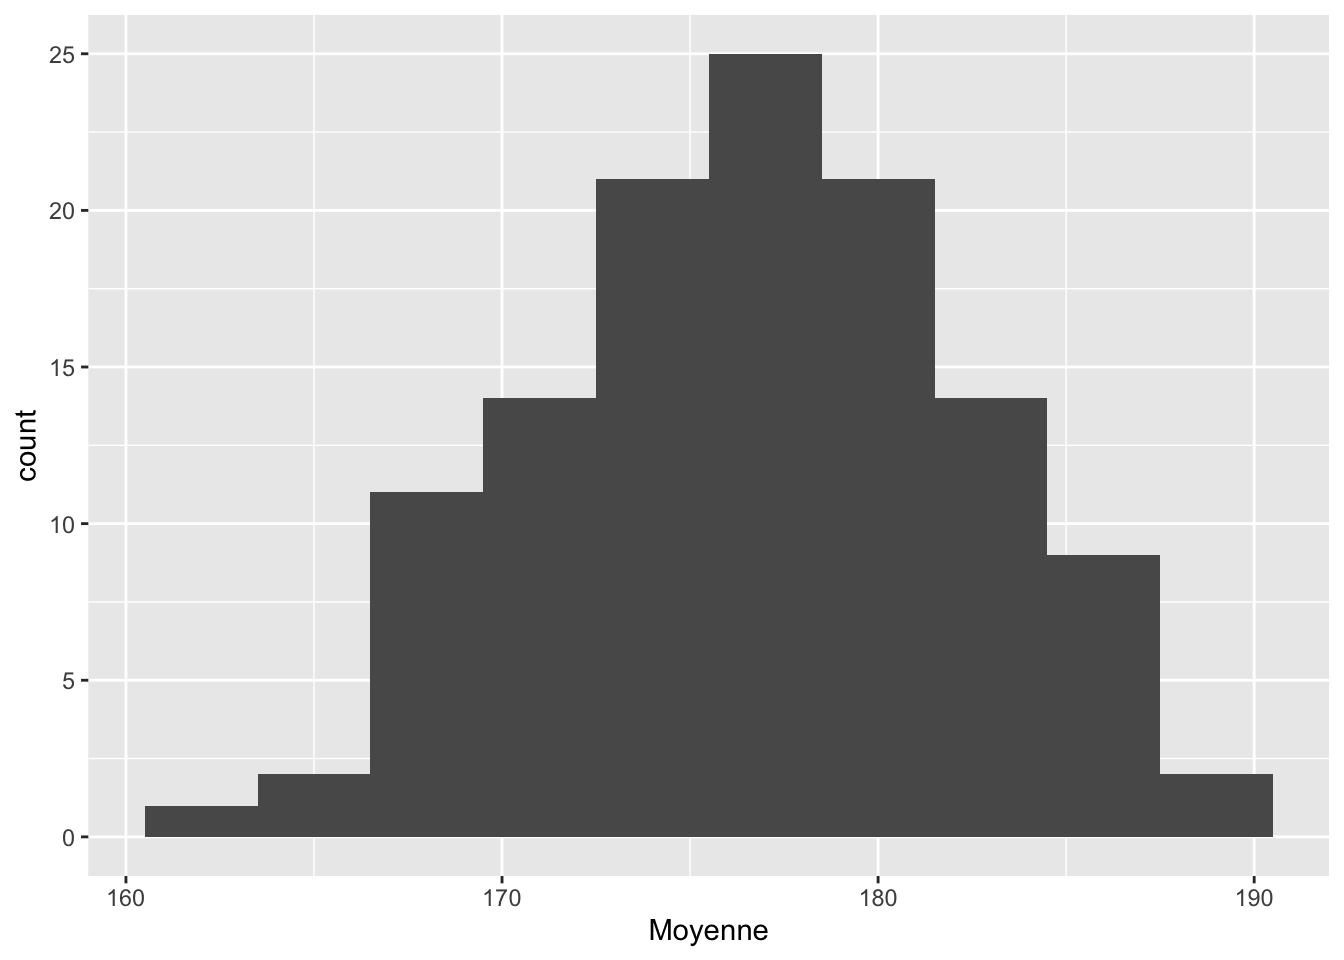
\includegraphics{_main_files/figure-latex/hist-1.pdf}
\caption{\label{fig:hist}Distribution d'échantillonage de la moyenne}
\end{figure}

\hypertarget{erreur-type}{%
\subsection{Erreur type}\label{erreur-type}}

Comment cette distribution nous aide-t-elle à savoir si la moyenne estimée à partir d'un échantillon \(\overline{X}\) est une bonne estimation de la moyenne de la population \(\mu\) ? Pour le savoir, on va d'abord admettre que la moyenne de cette distribution d'échantillonnage est la moyenne de la population. Ce qui permet alors de reformuler la question : on se demande alors quelle sera en moyenne la distance entre notre estimation \(\overline{X}\), qui est une valeur aléatoire de cette distribution, et la moyenne de la population \(\mu\).

Si vous vous souvenez du cours d'il y a deux semaines, il s'agit justement de la définition de l'\textbf{écart-type}, qui mesure un écart moyen à la moyenne. L'écart-type de la distribution d'échantillonnage de la moyenne (la distribution \ref{fig:hist}) nous donne donc l'erreur moyenne que l'on va réaliser en estimant la moyenne de la population \(\mu\) à l'aide de la moyenne de l'échantillon \(\overline{X}\). Il s'agit d'une grandeur importante, à laquelle on attribue le nom d'\textbf{erreur type}. Plus l'erreur type est importante, plus l'estimation réalisée à partir d'un échantillon sera en moyenne éloignée du paramètre que l'on cherche à mesurer.

Le problème, c'est qu'en général on ne va pas avoir accès à la distribution d'échantillonnage de la moyenne pour calculer l'erreur type, car on cherche justement à produire une estimation à partir de la seule connaissance d'un échantillon. Ici on doit utiliser un résultat de la théorie des probabilité, qui nous indique que si l'on fait l'hypothèse de l'indépendance statistique entre les différents individus de notre échantillon (ici que la taille d'un individu ne dépendra pas de la taille d'un autre), on peut estimer l'erreur type (notée SE, pour \emph{standard error}) comme \textbf{l'écart type de l'échantillon divisé par la racine carré de son effectif}.

\[ SE \approx \frac{s}{\sqrt{n}} \] où :

\begin{itemize}
\tightlist
\item
  \(s\) est l'écart type de l'échantillon
\item
  \(n\) l'effectif de l'échantillon
\end{itemize}

\hypertarget{thuxe9oruxe8me-central-limite}{%
\subsection{Théorème central limite}\label{thuxe9oruxe8me-central-limite}}

Ce résultat est une conséquence du \textbf{théorème central limite}, qui est un résultat fondamental de la théorie des probabilités, sans lequel il n'existerait pas de statistique inférentielle. Ce théorème indique que, pour toute variable quantitative de notre population (quelle que soit sa distribution), la distribution d'échantillonnage de la moyenne de cette variable va \emph{tendre vers} une loi normale de moyenne \(\mu\) et d'écart-type \(\sigma/{\sqrt{n}}\) lorsque la taille de l'échantillon augmente\footnote{`Tendre vers' renvoie à la notion de limite en mathématique. Si l'on considère une suite de nombres réels \(x_n\), on dit que la suite des valeurs (\(x_1, x_2, …, x_n\)) tend vers un nombre \(l\) si pour tout nombre \(\epsilon\) (aussi petit soit-il), il existe un nombre entier \(k\) telle que pour tout \(n > k\) on a \(x_n - l < \epsilon\). On dit alors que \(l\) est la limite de la suite \(x_n\) quand \(n\) tend vers l'infini, et on note \(\lim_{n\to\infty} x_n = l\). Par exemple, \(x_n = 1/n\) tend vers 0 : on le montre facilement à partir de la définition, car si on se donne un nombre \(\epsilon > 0\) (par exemple, 0,1) on sait que dès que \(n > 1/\epsilon\) (10 dans notre exemple), on aura \(x_n = 1/n < \epsilon\).}. En particulier, ce résultat permet de savoir que l'erreur que l'on va commettre, mesurée par l'écart-type de notre distribution d'échantillonnage, va diminuer lorsque n augmente. C'est un résultat relativement intuitif : plus la taille de l'échantillon augmente, plus l'estimateur (la moyenne de l'échantillon) sera proche du paramètre estimé (la moyenne de la population).

Formulé en termes abstraits, ce résultat peut être difficile à comprendre. Mais certaines représentations graphiques peuvent en donner une bonne intuition. Ci-dessous, on représente des distributions de probabilité pour un tirage aléatoire d'une pièce à pile ou face. On imagine qu'on réalise une série de tirages, en comptant 1 lorsqu'on obtient face et 0 sinon, puis on additionne tous les résultats. Les différentes courbes représentent les probabilités d'obtenir un total égal au chiffre indiqué en abscisses pour différents nombre de tirages. Lorsqu'on réalise un seul tirage, on a 50\% de chance d'obtenir 0 et 50\% de chance d'obtenir 1 (d'où le segment horizontal). Puis si on en fait un second, on a 25\% de chance d'obtenir deux fois pile (0), 25\% d'obtenir deux fois face (2), et 50\% d'obtenir une fois pile et une fois face (1). Et ainsi de suite.

\begin{figure}
\centering
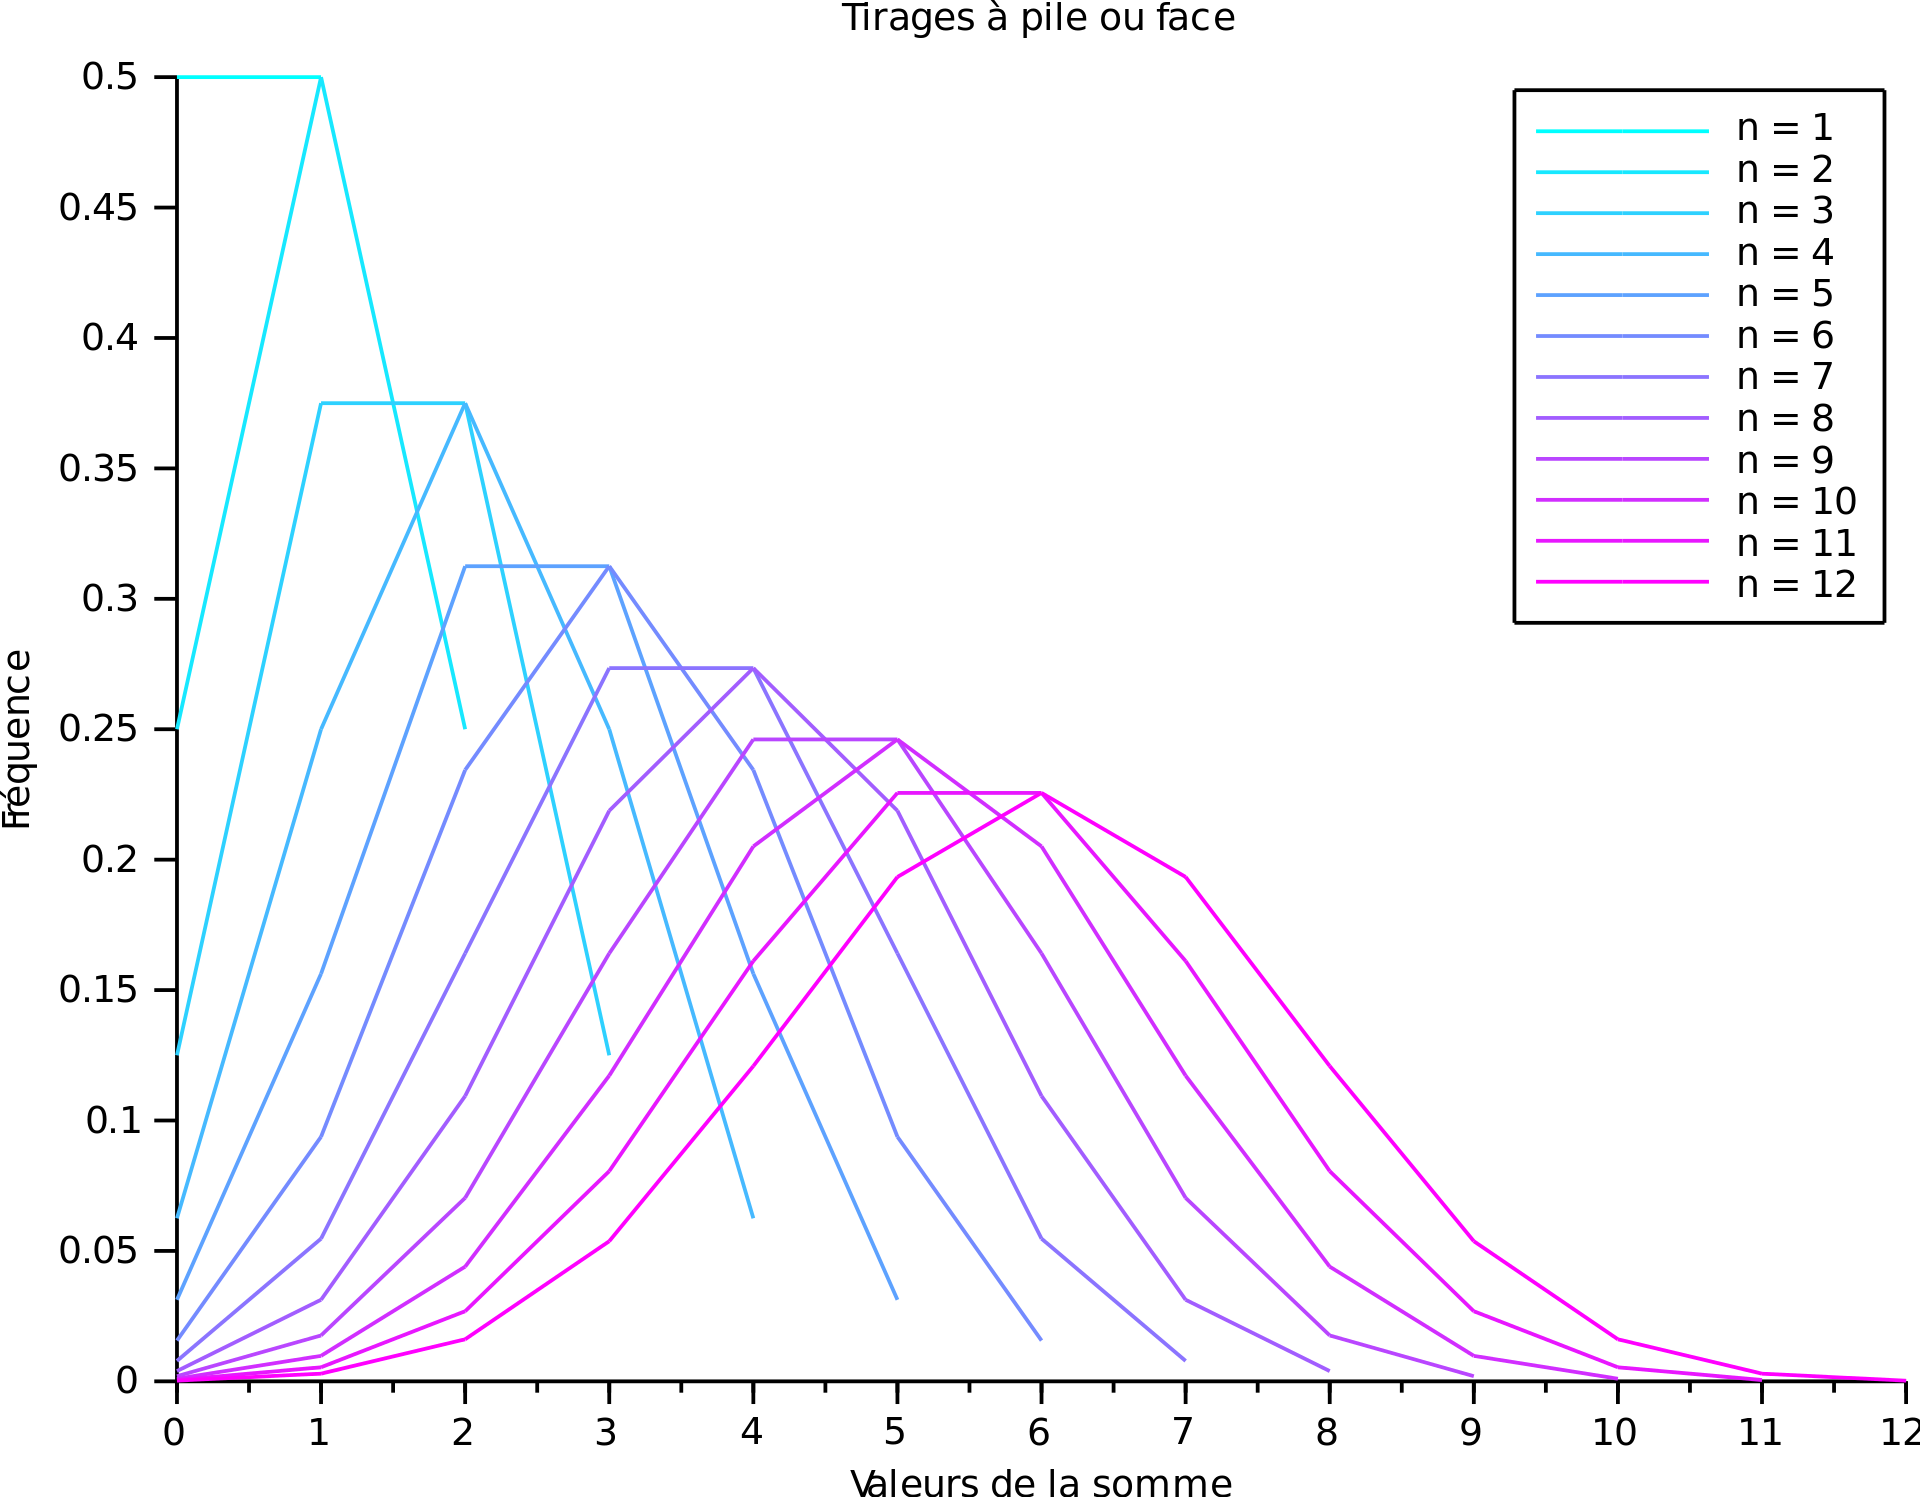
\includegraphics{images/tcl.png}
\caption{Fréquence d'apparition de la somme des valeurs d'un tirage alétaoire de 0 et 1}
\end{figure}

Remarquez qu'ici l'écart type de la distribution (la ``largeur'' de la cloche) augmente avec le nombre de tirages, car la distribution représentée correspond à la somme des valeurs obtenues et non à leur moyenne. Pour obtenir la distribution de la moyenne obtenue, il faudrait diviser la somme obtenu par le nombre de tirages : on obtiendrait alors des courbes entre 0 et 1, centrées sur 0,5, et dont l'écart-type diminue avec le nombre de tirages comme évoqué plus haut.

Cela permet d'avoir une bonne idée du résultat auquel on aboutirait si on cherchait à représenter les distributions d'échantillonnage d'une variable quantitative qui ne prend que deux valeurs, pour différentes tailles d'échantillon. Alors que la distribution de cette variable n'a rien de normale au sein de la population, la distribution d'échantillonnage deviendrait de plus en plus proche d'une loi normale à mesure que l'on augmenterait l'effectif de l'échantillon.

\hypertarget{intervalles-de-confiance}{%
\section{Intervalles de confiance}\label{intervalles-de-confiance}}

\hypertarget{z-distribution}{%
\subsection{\texorpdfstring{\emph{z}-distribution}{z-distribution}}\label{z-distribution}}

Le théorème central limite permet donc d'estimer l'erreur type d'une variable quantitative relative à des données produites sur un échantillon, et donc de quantifier l'incertitude des grandeurs mesurées lorsqu'il s'agit de les généraliser à l'ensemble de la population. On souhaiterait maintenant avoir un moyen de présenter cette incertitude de manière la plus explicite possible. Pour cela, on va utiliser les propriétés de la loi normale.

Comme nous l'avons évoqué dans l'avant dernier cours (section \ref{loi-normale}), lorsque l'on sait qu'une variable est distribuée de manière normale, on peut connaître la probabilité qu'une valeur sélectionnée de manière aléatoire se trouve à moins d'une certaine distance de la moyenne. Par exemple, 99\% des valeurs se situent à moins de 2,58 écart-type de la moyenne. Ces chiffres permettent de préciser des \textbf{intervalles de confiance} relatifs à une estimation. On va dire qu'on est la moyenne \(\mu\) se trouve dans l'intervalle \([\overline{X}-2,58*SE \;;\; \overline{X}+2,58*SE]\) avec une certitude de 99\%.

Disons maintenant que l'on cherche l'intervalle de confiance à 95\% plutôt qu'à 99\%. Comment l'obtenir ? Pour cela on définit parfois à partir de notre distribution d'échantillonnage une nouvelle distribution que l'on nomme \emph{z}-distribution de cette manière :

\[ z = \frac{\overline{X} - \mu}{SE} = \frac{\overline{X} - \mu}{\sigma/\sqrt{n}}\]

Si \(\overline{X}\) est distribuée selon une loi normale de moyenne \(\mu\) et d'écart-type \(SE = \sigma/\sqrt{n}\), alors \(z\) sera distribuée selon une loi normale de moyenne 0 et d'écart-type égal à 1, ce qu'on appelle la \textbf{loi normale centrée réduite}. C'est une manière de toujours se ramener à la même distribution. On parle de \textbf{standardisation}. En se ramenant à une loi normale, on peut donc obtenir à partir d'une table de valeurs l'équivalent du chiffre 2,58 pour n'importe quelle pourcentage de certitude attendu.

Dans R, la fonction \texttt{qnorm()} permet par exemple d'obtenir ces valeurs :

\begin{Shaded}
\begin{Highlighting}[]
\FunctionTok{qnorm}\NormalTok{(}\AttributeTok{p =} \FloatTok{0.975}\NormalTok{)}
\end{Highlighting}
\end{Shaded}

\begin{verbatim}
## [1] 1.959964
\end{verbatim}

Cette fonction permet de déterminer n'importe quel quantile de la loi normale centrée réduite. C'est-à-dire qu'elle donne ici la valeur qui sépare les 97,5\% de valeurs les plus faibles des 2,5\% les plus élevées. On utilise 97,5\% plutôt que 95\% on souhaite également délimiter les 2,5\% des valeurs les plus faibles. Comme la courbe est symétrique par rapport à 0, la valeur équivalente sera toujours l'opposé de celle cherchée ici. On peut le vérifier :

\begin{Shaded}
\begin{Highlighting}[]
\FunctionTok{qnorm}\NormalTok{(}\AttributeTok{p =} \FloatTok{0.025}\NormalTok{)}
\end{Highlighting}
\end{Shaded}

\begin{verbatim}
## [1] -1.959964
\end{verbatim}

Graphiquement, les deux valeurs obtenues permettent de délimiter 95\% de l'aire comprise sous le graphe de la loi normale centrée réduite. Sur le graphique suivant, on représente en rouge les 2,5\% de l'aire sous la courbe qui représentent les valeurs extrêmes de la distribution.

\begin{figure}
\centering
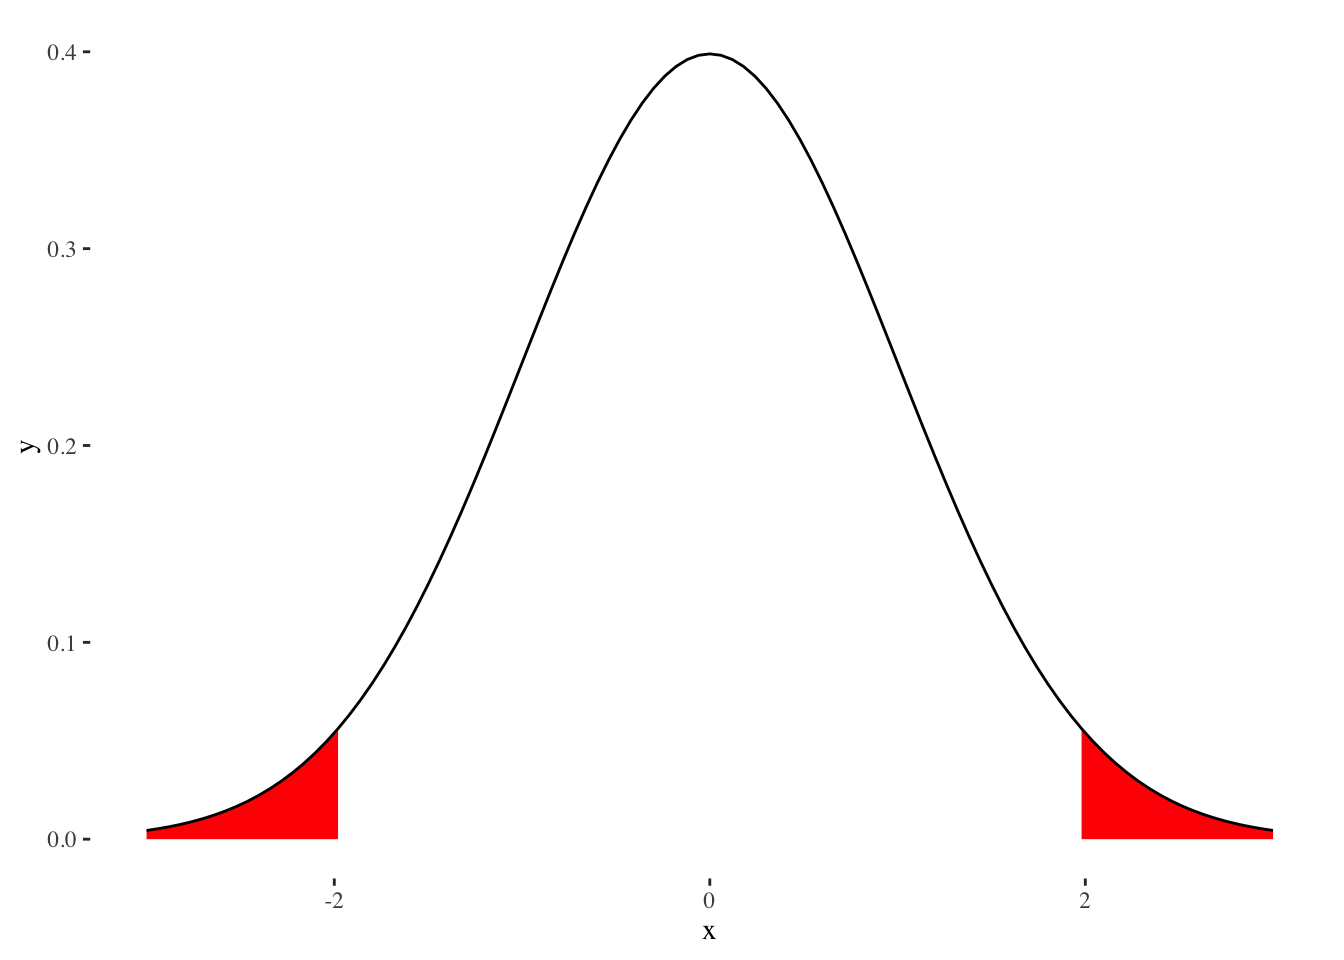
\includegraphics{_main_files/figure-latex/unnamed-chunk-35-1.pdf}
\caption{\label{fig:unnamed-chunk-35}Représentation graphique de la loi normale centrée réduite, et en rouge des 5\% de l'aire sous la courbe situées aux deux extrêmes de la distribution}
\end{figure}

\hypertarget{t-distribution}{%
\subsection{\texorpdfstring{\emph{t}-distribution}{t-distribution}}\label{t-distribution}}

En réalité, cette manière d'estimer un intervalle de confiance n'est pas la plus précise. Nous avons vu plus haut que \(SE \approx s/\sqrt{n}\), où s est l'écart-type de l'échantillon et n son effectif. Les statisticiens ont montré que cette approximation n'est pas la meilleure estimation de l'erreur-type. D'après le théorème central limite, on sait que l'erreur type est égale à \(SE = \sigma/\sqrt{n}\) où \(\sigma\) est l'écart-type de la population. L'approximation qui est discutable est donc celle qui consiste à estimer l'erreur type \(\sigma\) par la valeur \(s/\sqrt{n}\).

C'est ici qu'on peut préciser la différence entre \textbf{statistique} et \textbf{estimateur}. Une statistique est la valeur mesurée sur notre échantillon, par exemple l'écart-type de l'échantillon \(s\). Lorsqu'on parle d'estimateur, on sous-entend que l'on cherche la meilleure estimation possible d'un paramètre à partir des données de l'échantillon. Il existe des bons et des mauvais estimateurs. Un critère souvent utilisé est celui de la moyenne de l'estimateur lorsqu'on réalise plusieurs échantillons. Si il prend en moyenne la valeur que l'on cherche à estimer, on parle alors d'un estimateur \textbf{non biaisé}. Un exemple d'un tel estimateur est la moyenne de l'échantillon \(\overline{X}\). Dans ce cas, \(\overline{X}\) désigne à la fois la moyenne statistique de notre échantillon, et notre estimation de la moyenne de la population.

Contrairement à la moyenne, l'écart-type observé \(s\) n'est pas un bon estimateur de l'écart-type \(\sigma\). Pour une raison que l'on ne développera pas, il faut remplacer n par n-1 dans la définition de l'écart-type pour obtenir un estimateur non biaisé.

\[ \hat{\sigma} = \sqrt{\frac{1}{n-1}\sum_{i=1}^n{(X_i - \overline{X})}}\]

Remarquez qu'ici, on doit utiliser deux notations différentes pour désigner l'écart type de notre échantillon \(s\) et l'estimateur de l'écart-type \(\hat{\sigma}\) (les estimateurs sont souvent écrits avec un chapeau). On appelle alors \(n-1\) le nombre de \textbf{degrés de libertés} de l'estimation. Lorsqu'on ne connaît pas l'écart-type \(\mu\) de la population, il faut donc utiliser plutôt que la distribution \emph{z} ce qu'on appelle la \emph{t}-distribution (parfois aussi nommée ``t de Student'') :

\[ t = \frac{\overline{X} - \mu}{\hat{\sigma}/\sqrt{n}}\]

La distribution \emph{t} est très proche de la loi normale, mais dépend du nombre de degré de libertés de la distribution (égal à \(n-1\)). Comme pour la loi normale, on peut lire les valeurs que l'on cherche à partir d'un \href{https://www.sjsu.edu/faculty/gerstman/StatPrimer/t-table.pdf}{table}, ou bien en utilisant la fonction \texttt{qt()} dans R. La table en lien permet de voir comment varie \emph{t} avec le nombre de degrés de liberté (en lisant les données d'une même colonne). Vous pouvez voir que, pour chaque degré de certitude, par exemple 90\%, la valeur \(t_{90}\) diminue avec le nombre de degrés de libertés. En bas du tableau est représenté les valeurs de \emph{z} associées. On peut remarquer que \emph{t} et \emph{z} sont très différentes pour les faibles effectifs, mais dès que le nombre de degrés de liberté augmente (par exemple df = 100), leurs valeurs sont très proches.

\hypertarget{un-exemple}{%
\subsection{Un exemple}\label{un-exemple}}

Prenons la base de données \texttt{hdv2003} du package \texttt{questionr}. On va prendre l'ensemble des individus de cette base comme population de référence, et échantillonner aléatoirement 20 individus de cette base de données. On souhaite estimer le temps moyen quotidien passé devant la télévision avec un intervalle de confiance à 95\%.

Voici les valeurs de la variable \texttt{heures.tv} pour les 20 individus et leur moyenne :

\begin{Shaded}
\begin{Highlighting}[]
\NormalTok{d}\SpecialCharTok{$}\NormalTok{heures.tv}
\end{Highlighting}
\end{Shaded}

\begin{verbatim}
##  [1] 3.0 2.0 7.0 0.0 2.0 0.0 2.0 4.0 4.0 1.0 0.3 3.0 3.0 5.0 3.0 1.0 0.0 2.0 2.1
## [20] 2.0
\end{verbatim}

\begin{Shaded}
\begin{Highlighting}[]
\FunctionTok{mean}\NormalTok{(d}\SpecialCharTok{$}\NormalTok{heures.tv)}
\end{Highlighting}
\end{Shaded}

\begin{verbatim}
## [1] 2.32
\end{verbatim}

Il faut aussi calculer l'estimation de l'erreur type :

\begin{Shaded}
\begin{Highlighting}[]
\FunctionTok{sd}\NormalTok{(d}\SpecialCharTok{$}\NormalTok{heures.tv)}\SpecialCharTok{*}\FunctionTok{sqrt}\NormalTok{(}\DecValTok{1}\SpecialCharTok{/}\DecValTok{19}\NormalTok{)}
\end{Highlighting}
\end{Shaded}

\begin{verbatim}
## [1] 0.4105668
\end{verbatim}

On ne connaît pas l'écart-type de la population, on doit donc utiliser la \emph{t}-distribution. Comme \(n=20\), on a \(df = 20 - 1 = 19\). On peut utiliser cette \href{https://www.sjsu.edu/faculty/gerstman/StatPrimer/t-table.pdf}{table} et lire les valeurs associées à \(t_{.975}\), en sélectionnant la ligne \(df = 19\) et ``two tails'' (car on cherche un intervalle symétrique). On lit directement la valeur \(t_{.975} = 2.093\). Autrement, on peut utiliser la fonction \texttt{qt()} :

\begin{Shaded}
\begin{Highlighting}[]
\FunctionTok{qt}\NormalTok{(}\AttributeTok{p =} \FloatTok{0.975}\NormalTok{, }\AttributeTok{df =} \DecValTok{19}\NormalTok{)}
\end{Highlighting}
\end{Shaded}

\begin{verbatim}
## [1] 2.093024
\end{verbatim}

On obtient (heureusement) la même valeur. Cela nous permet d'établir notre intervalle de confiance à 95\% :

\[ I_{95} = [2,32-0,41*2,093 \;;\;  2,32 + 0,41*2,093] = [1,46 \;;\; 3,18] \]
Finalement, notre intervalle de confiance de la moyenne va de 1,46 à 3,18 heures passées à regarder la télévision. Si l'on souhaite une estimation plus précise, on peut prendre un échantillon plus grand. Le code suivant réalise les mêmes calculs avec un échantillon de 200 individus :

\begin{Shaded}
\begin{Highlighting}[]
\CommentTok{\# On sélectionne alétaoirement 1/10 de la population, c\textquotesingle{}est{-}à{-}dire 200 individus}
\NormalTok{d2 }\OtherTok{\textless{}{-}}\NormalTok{ hdv2003 }\SpecialCharTok{\%\textgreater{}\%} \FunctionTok{sample\_frac}\NormalTok{(}\FloatTok{0.1}\NormalTok{)}
\CommentTok{\# On calcule directement la borne inférieures de notre intervalle de confiance}
\FunctionTok{mean}\NormalTok{(d2}\SpecialCharTok{$}\NormalTok{heures.tv, }\AttributeTok{na.rm =}\NormalTok{ T) }\SpecialCharTok{{-}} \FunctionTok{qt}\NormalTok{(}\AttributeTok{p=} \FloatTok{0.975}\NormalTok{, }\AttributeTok{df =} \DecValTok{199}\NormalTok{) }\SpecialCharTok{*} \FunctionTok{sd}\NormalTok{(d2}\SpecialCharTok{$}\NormalTok{heures.tv, }\AttributeTok{na.rm =}\NormalTok{ T)}\SpecialCharTok{*}\FunctionTok{sqrt}\NormalTok{(}\DecValTok{1}\SpecialCharTok{/}\DecValTok{199}\NormalTok{)}
\end{Highlighting}
\end{Shaded}

\begin{verbatim}
## [1] 2.082967
\end{verbatim}

\begin{Shaded}
\begin{Highlighting}[]
\CommentTok{\# Et la borne supérieure}
\FunctionTok{mean}\NormalTok{(d2}\SpecialCharTok{$}\NormalTok{heures.tv, }\AttributeTok{na.rm =}\NormalTok{ T) }\SpecialCharTok{+} \FunctionTok{qt}\NormalTok{(}\AttributeTok{p=} \FloatTok{0.975}\NormalTok{, }\AttributeTok{df =} \DecValTok{199}\NormalTok{) }\SpecialCharTok{*} \FunctionTok{sd}\NormalTok{(d2}\SpecialCharTok{$}\NormalTok{heures.tv, }\AttributeTok{na.rm =}\NormalTok{ T)}\SpecialCharTok{*}\FunctionTok{sqrt}\NormalTok{(}\DecValTok{1}\SpecialCharTok{/}\DecValTok{199}\NormalTok{)}
\end{Highlighting}
\end{Shaded}

\begin{verbatim}
## [1] 2.614033
\end{verbatim}

On peut observer que l'intervalle de confiance à 95\% est plus réduit, il s'agit donc d'une meilleure estimation. Finalement, on peut calculer la moyenne recherchée :

\begin{Shaded}
\begin{Highlighting}[]
\FunctionTok{mean}\NormalTok{(hdv2003}\SpecialCharTok{$}\NormalTok{heures.tv, }\AttributeTok{na.rm =} \ConstantTok{TRUE}\NormalTok{)}
\end{Highlighting}
\end{Shaded}

\begin{verbatim}
## [1] 2.246566
\end{verbatim}

Remarquez qu'on doit utiliser l'argument \texttt{na.rm\ =\ TRUE} dans la fonction \texttt{mean()} en raison de l'existence de valeurs manquantes dans la variable \texttt{heures.tv}.

\hypertarget{interpruxe9ter-un-intervalle-de-confiance}{%
\subsection{Interpréter un intervalle de confiance}\label{interpruxe9ter-un-intervalle-de-confiance}}

Une fois que l'on a calculé l'intervalle de confiance, le dernier problème est de savoir exactement quelle signification lui attribuer. On pourrait être tenté de dire ``la moyenne que l'on essaie d'estimer a 95\% de chance d'être dans l'intervalle''. Mais ça n'est pas vraiment une bonne formulation, car la moyenne à estimer n'est pas aléatoire : soit elle est dans l'intervalle soit elle ne l'est pas, donc la probabilité qu'elle soit dans entre les deux bornes de l'intervalle est 0 (elle n'y est pas) ou 1 (elle y est) mais pas 0,95. Ce qui est aléatoire ici, c'est l'intervalle que l'on a estimé et non la moyenne \(\mu\). Il faudrait donc plutôt dire que ``l'intervalle a 95\% de chance de capturer la moyenne entre ses bornes''. Autrement dit, si l'on calcule 100 intervalles de confiance à 95\% (quels qu'ils soient, pas nécessairement sur la même distribution), on aura en moyenne 5 intervalles qui ne captureront pas la moyenne \(\mu\).

\hypertarget{analyse-bivariuxe9e-et-corruxe9lation-ii}{%
\chapter{Analyse bivariée et corrélation II}\label{analyse-bivariuxe9e-et-corruxe9lation-ii}}

Jusqu'à maintenant, on a passé en revue :

\begin{itemize}
\tightlist
\item
  l'étude univariée d'une variable qualitative ou d'une variable quantitative (cours \ref{univar} et \ref{infer}).
\item
  l'étude de la corrélation entre deux variables qualitatives (cours \ref{cor1})
\end{itemize}

Le cours de cette semaine est destiné à présenter les notions
essentielles impliquées dans l'étude de la corrélation entre plusieurs
variables quantitatives. La première partie du cours présente la
représentation graphique associée à une telle étude, la notion de
covariance et le modèle de la régression linéaire, tandis que la seconde
partie aborde les questions d'inférence statistique avec la présentation
d'un nouveau test d'hypothèse, le \emph{t}-test.

\hypertarget{deux-variables-quantitatives}{%
\section{Deux variables quantitatives}\label{deux-variables-quantitatives}}

Étudier la corrélation entre deux variables quantitatives permet en
général d'utiliser un plus grand nombre d'outils que l'étude des
variables qualitatives, car il est possible de faire des calculs à
partir des modalités des variables considérées. Certaines
représentations graphiques sont aussi plus adaptées à l'étude des
variables quantitatives.

\hypertarget{repruxe9senter-deux-variables-quantitatives}{%
\subsection{Représenter deux variables quantitatives}\label{repruxe9senter-deux-variables-quantitatives}}

Lorsqu'on souhaite observer les liens entre deux variables
quantitatives, on représente en général un \textbf{nuage de points}. Il
s'agit d'un graphique dans lequel chacune des variables est représentée
selon un axe (l'une en abscisses, l'autre en ordonnées), ce qui permet de
positionner chaque individu statistique à partir des valeurs associées à
chacune des variables, qui seront alors ses coordonnées dans le plan.

\begin{Shaded}
\begin{Highlighting}[]
\FunctionTok{ggplot}\NormalTok{(USArrests) }\SpecialCharTok{+} \FunctionTok{geom\_point}\NormalTok{(}\FunctionTok{aes}\NormalTok{(}\AttributeTok{x =}\NormalTok{ Murder, }\AttributeTok{y =}\NormalTok{ Rape))}
\end{Highlighting}
\end{Shaded}

\begin{figure}
\centering
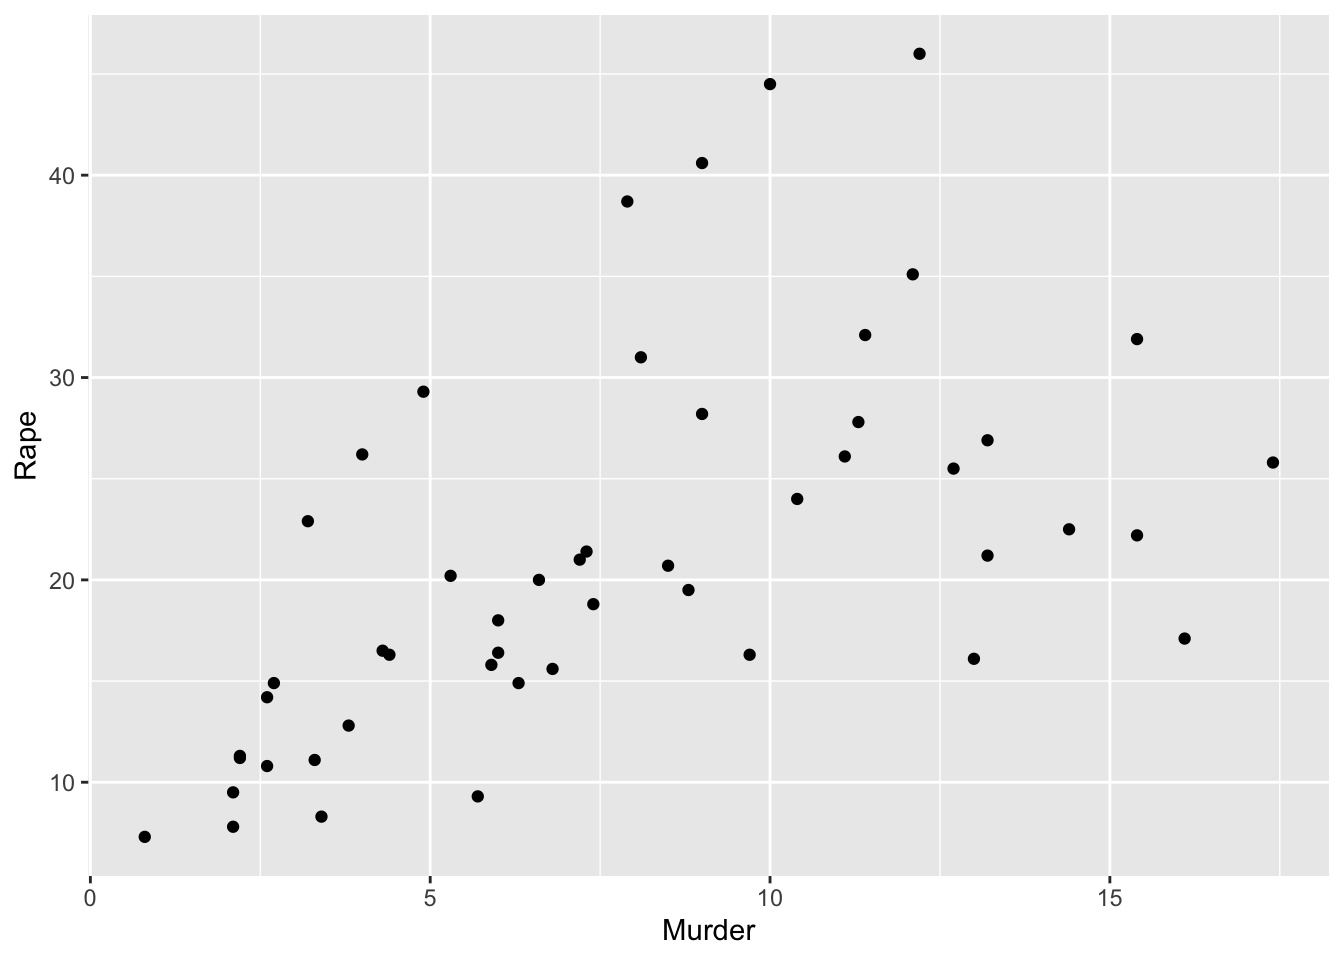
\includegraphics{_main_files/figure-latex/arrests-1.pdf}
\caption{\label{fig:arrests}Un exemple à partir des données USArrests : chaque point représente un état des États-Unis, dont la position dépend de son taux d'arrestation pour meurtres (pour 100~000 habitants, selon x) et pour viol (pour 100~000 habitants, selon y) en 1974}
\end{figure}

Sur cet exemple, chaque point représente un État des États-Unis. Plus le
point est situé à droite du graphe, plus le taux d'arrestation pour
meurtre correspondant est important. De même, plus il est situé en hauteur sur le graphe, plus le taux d'arrestation pour viol est important (les données
datent de 1974).

Pour avoir une idée d'où se situent les différents État sur le graphe,
on peut indiquer sur le graphe à côté de chaque point l'État auquel il
correspond.

\begin{verbatim}
## Warning: ggrepel: 1 unlabeled data points (too many overlaps). Consider
## increasing max.overlaps
\end{verbatim}

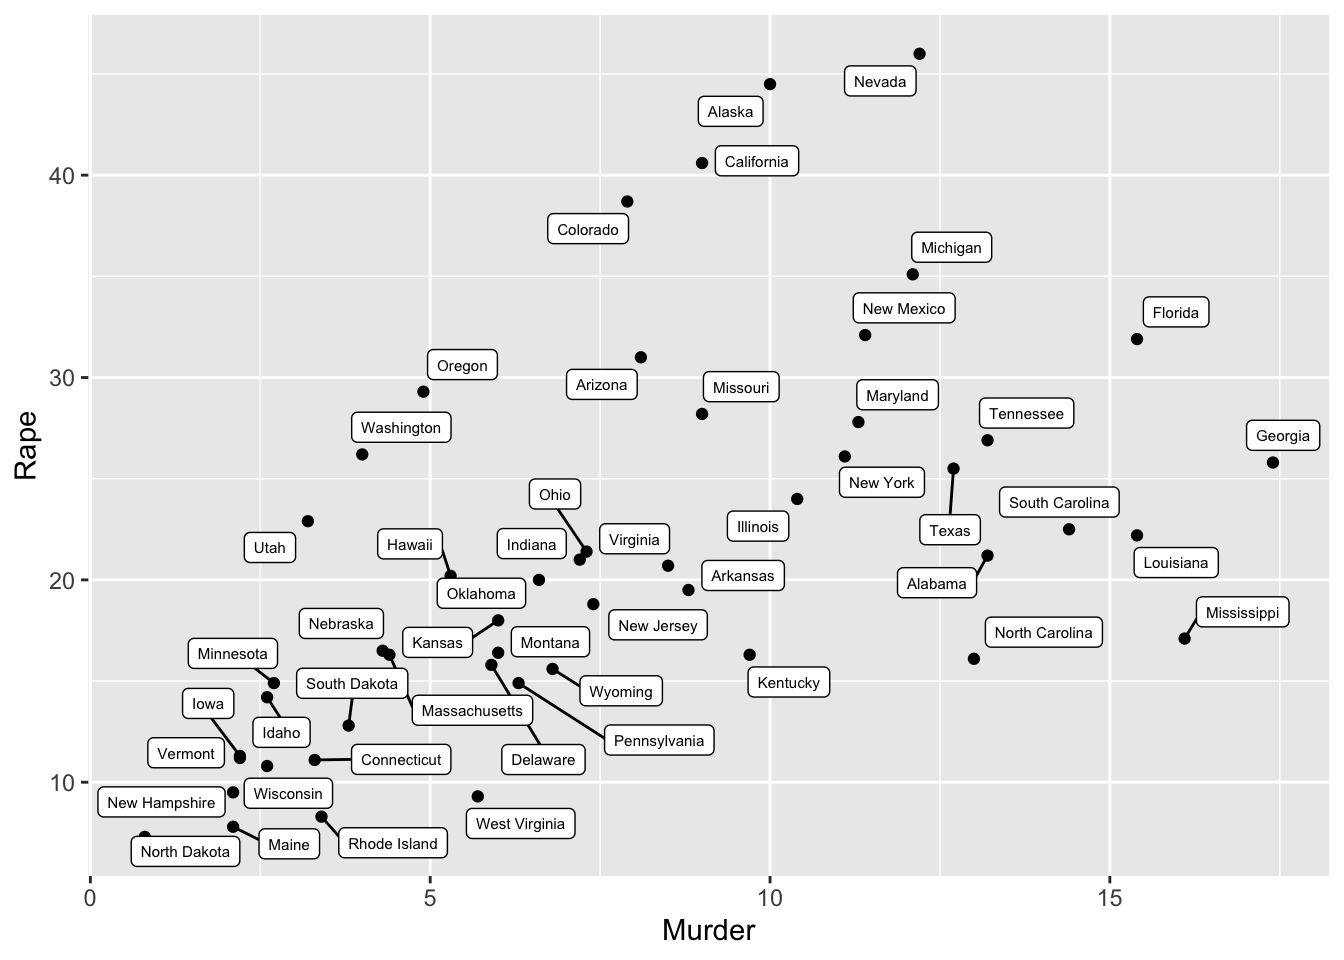
\includegraphics{_main_files/figure-latex/unnamed-chunk-43-1.pdf}

La forme du nuage de point permet caractériser le lien entre les
variables : on observe ici qu'il y a peu d'État dans en haut à gauche ou
en bas à droite du graphique. C'est-à-dire que lorsque le taux
d'arrestation pour meurtre est faible dans un État, le taux
d'arrestation pour viol l'est aussi. Il semble donc exister un lien de
corrélation entre ces deux variables : lorsqu'une augmente, on observe
en général que l'autre augmente également.

\hypertarget{la-covariance}{%
\subsection{La covariance}\label{la-covariance}}

La covariance est une grandeur qui permet de mesurer la corrélation
entre deux variables quantitatives. C'est une généralisation de la
variance dans le cas de deux variables. Elle mesure la moyenne du
produit des écarts à la moyenne de deux variables X et Y :

\[ Cov(X, Y) = \frac{1}{N} \sum^N_{i = 1}(X_i - \bar{X})(Y_i - \bar{Y})\]
On peut remarquer immédiatement que \(Cov(X,X) = Var(X)\), donc il s'agit
bien d'une généralisation de la variance.

Pourquoi la covariance mesure-t-elle une corrélation entre X et Y ? On
peut le comprendre à partir d'un exemple. Disons que X mesure la taille
d'un individu i, et Y son poids. Lorsque X est supérieur à sa moyenne, on
aura par définition \((X_i - \overline{X}) > 0\). Mais les personnes les
plus grandes seront aussi en moyenne plus lourdes que la moyenne, donc
on aura le plus souvent \((Y_i - \overline{Y}) > 0\). À l'inverse, les
personnes qui sont plus petites que la moyenne seront aussi en moyenne
plus légères, donc lorsque \((X_i - \overline{X}) < 0\) on aura la plupart
du temps \((Y_i - \overline{Y}) < 0\). Les écarts à la moyenne de X et Y
auront donc le plus souvent le même signe, leur produit sera donc
positif. Autrement dit, une corrélation positive entre les deux
variables (c'est-à-dire le fait qu'une augmentation de X est
généralement associée à une augmentation de Y) a pour conséquence une
covariance positive. On pourrait montrer de la même manière qu'une
corrélation négative induit une covariance inférieure à 0. Enfin,
lorsque la covariance de X et Y est nulle, on dit que les deux variables
sont \textbf{indépendantes} : la valeur de l'une n'a en moyenne pas de lien
avec la valeur de l'autre.

La covariance permet donc de retranscrire numériquement l'idée de
corrélation. On peut par exemple la calculer pour les deux variables \texttt{Murder}
et \texttt{Rape} représentées plus haut (figure \ref{fig:arrests}).

\begin{Shaded}
\begin{Highlighting}[]
\FunctionTok{cov}\NormalTok{(USArrests}\SpecialCharTok{$}\NormalTok{Murder, USArrests}\SpecialCharTok{$}\NormalTok{Rape)}
\end{Highlighting}
\end{Shaded}

\begin{verbatim}
## [1] 22.99141
\end{verbatim}

On obtient bien un coefficient positif, comme le suggérait l'allure du nuage de
points représenté. Le problème avec la covariance, c'est qu'au delà de
son signe il est difficile de lui attribuer une signification. Cela est
du fait que sa valeur dépend des unités de \(X\) et de \(Y\). On préfèrerait
un indice compris entre \(-1\) et \(1\).

Pour l'obtenir, on calcule ce qu'on appelle \textbf{le coefficient de corrélation de Pearson}. Il règle le problème de l'unité de la covariance en la divisant par les écarts types de \(X\) et de \(Y\) :

\[ r_{XY} = \frac{Cov(X,Y)}{\sigma_{\bar{X}}\sigma_{\bar{Y}}} \]

En normalisant la covariance, on conserve ses propriétés intéressantes,
mais on obtient un indicateur plus facile à interpréter. Lorsque le
coefficient de corrélation est égal à 1, les deux variables sont
parfaitement corrélées. Si l'on représente leur nuage de points, on doit
voir une droite de pente positive. À l'inverse, un coefficient de
corrélation égal à -1 correspond à une droite de pente négative. Le coefficient mesure donc l'intensité de la corrélation : s'il est proche de 0, les variables sont faiblement corrélées, s'il est proche de 1 ou de -1, elle le sont fortement. Voici
le résultat qu'on obtient pour notre exemple :

\begin{Shaded}
\begin{Highlighting}[]
\FunctionTok{cov}\NormalTok{(USArrests}\SpecialCharTok{$}\NormalTok{Murder, USArrests}\SpecialCharTok{$}\NormalTok{Rape)}\SpecialCharTok{/}\NormalTok{(}\FunctionTok{sd}\NormalTok{(USArrests}\SpecialCharTok{$}\NormalTok{Murder)}\SpecialCharTok{*}\FunctionTok{sd}\NormalTok{(USArrests}\SpecialCharTok{$}\NormalTok{Rape))}
\end{Highlighting}
\end{Shaded}

\begin{verbatim}
## [1] 0.5635788
\end{verbatim}

\hypertarget{la-regression-linuxe9aire}{%
\section{La regression linéaire}\label{la-regression-linuxe9aire}}

La méthode de la régression linéaire consiste à modéliser la relation
entre deux variable quantitative par une droite, et cela même lorsque le
coefficient de corrélation entre ces deux variables n'est pas égal à 1
ou -1. Graphiquement, il s'agit de trouver la droite qui résume le mieux
le lien entre les deux variables.

Dans cette partie, on prendra comme exemple le jeu de données fictives \texttt{parenthood} proposé par Dan Navarro \citep{navarro2015}. Il contient plusieurs
variables. L'une d'entre elles est le ``niveau de mauvaise humeur de Dan''
: on imagine qu'il le note chaque jour, en lui attribuant un score entre
0 et 100 (0 lorsqu'il est parfaitement de bonne humeur, 100 lorsqu'il est parfaitement de mauvaise humeur). La seconde variable que l'on va utiliser est son temps de sommeil.

\begin{figure}
\centering
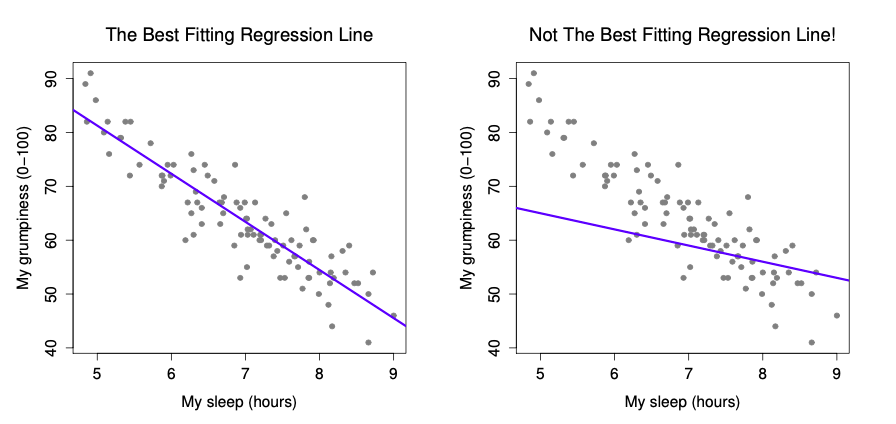
\includegraphics{images/regressionline.png}
\caption{L'objectif est de trouver la droite qui résume le mieux le nuage de
points. À gauche, la meilleure regression, à droite, une autre beaucoup
moins bien}
\end{figure}

Vous pouvez remarquer que les deux variables n'ont pas vraiment le même
statut. La question que l'on va se poser est \textbf{l'effet du temps de sommeil sur la mauvaise humeur de Dan}. On dit que la variable ``mauvaise humeur''
est la \textbf{variable à expliquer}, tandis que la variable ``temps de sommeil''
est la \textbf{variable explicative}.

\hypertarget{principe-de-la-ruxe9gression}{%
\subsection{Principe de la régression}\label{principe-de-la-ruxe9gression}}

Comme il s'agit de modéliser la relation entre ces variables par une ligne droite, commençons par écrire l'équation d'une ligne droite :

\[ y = ax + b \]

\(y\) et \(x\) sont deux variables, et \(a\) et \(b\) deux coefficients : ce sont les nombres que l'on cherche à déterminer. On peut remarquer que l'asymétrie entre les deux variables se retrouve dans l'équation : \(y\) est la variable à expliquer, et \(x\) la variable explicative.

\begin{itemize}
\tightlist
\item
  \(a\) est la \textbf{pente} de la droite (c'est-à-dire l'augmentation de
  \(y\) lorsque \(x\) augmente d'une unité)
\item
  \(b\) est \textbf{l'ordonnée à l'origine} (c'est-à-dire la valeur de \(y\)
  quand \(x = 0\))
\end{itemize}

La formule qu'on utilise pour décrire une droite de régression est très
similaire :

\[ \hat{Y}_i = b_1X_i + b_0\]

\begin{itemize}
\tightlist
\item
  on note \(X_i\) et \(Y_i\) plutôt que \(X\) et \(Y\) pour bien indiquer que cette relation est valable pour chacune des observations
\item
  on note \(\hat{Y}_i\) plutôt que \(Y_i\), pour faire la différence entre les valeurs observées \(Y_i\), et les valeurs estimées \(\hat{Y}_i\), ce sont les valeurs qui sont prédites à partir du modèle.
\item
  on note les coefficients \(b_1\) et \(b_0\) plutôt que \(a\) et \(b\) (ce qui permettra plus tard d'ajouter \(b_2\), \(b_3\), etc.).
\end{itemize}

Puisque notre estimation n'est pas parfaite, c'est-à-dire qu'elle
diffère des données observées, il existe une différence entre les
données observées et les données estimées qu'on appelle \textbf{résidus} :

\[ \epsilon_i = Y_i - \hat{Y}_i\]
L'expression des résidus permet de réécrire l'équation du modèle de cette manière :

\[ Y_i = b_1X_i + b_0 + \epsilon_i \]
La question est alors de savoir quel critère retenir lorsqu'on cherche ``la meilleure droite de régression''. La figure suivante représente la grandeur des résidus pour deux droites de régression. Sur la gauche, on a l'intuition que la droite est une meilleure estimation du nuage de points : les résidus sont aussi en moyenne plus faibles.

\begin{figure}
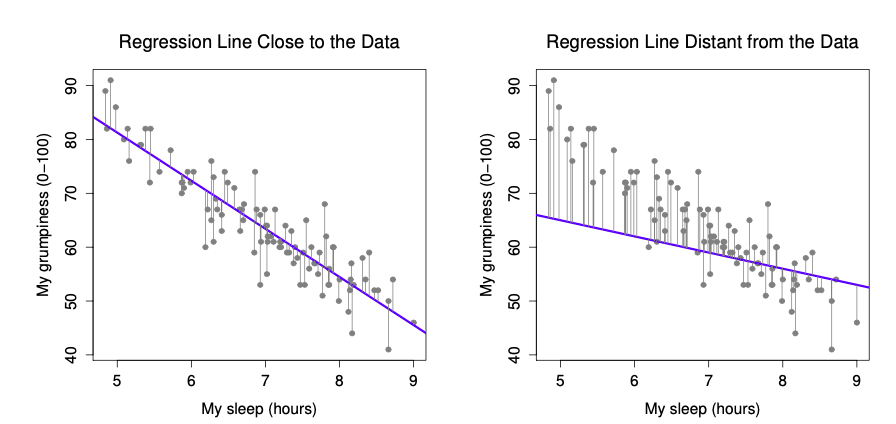
\includegraphics[width=12.44in]{images/residuals} \caption{Une représentation graphique des résidus associés aux deux droites de régression. On remarque que les résidus sont moins grands en moyenne dans le premier cas que dans le second}\label{fig:residus}
\end{figure}

\hypertarget{estimer-une-droite-de-regression}{%
\subsection{Estimer une droite de regression}\label{estimer-une-droite-de-regression}}

C'est ce critère que l'on va retenir pour déterminer quelle est la meilleure droite de régression. Les coefficients estimés, \(b_0\) et \(b_1\) sont ainsi ceux qui minimisent la somme des carrés des résidus, qu'on peut écrire :

\[ \sum^{N}_{i = 1} (Y_i- \hat{Y}_i)^2 \]

ou encore :

\[ \sum^{N}_{i = 1} \epsilon_i^2 \]

On appelle cette méthode d'estimation des coefficients la \textbf{méthode des moindres carrés ordinaires}. Trouver les coefficients qui minimisent la somme des carrés des résidus est un problème purement mathématique. L'idée est que vous n'avez pas besoin de savoir comment faire, mais que R peut le faire pour vous à l'aide de la fonction \texttt{lm()}.

\hypertarget{utiliser-la-fonction-lm-dans-r}{%
\subsection{\texorpdfstring{Utiliser la fonction \texttt{lm()} dans R}{Utiliser la fonction lm() dans R}}\label{utiliser-la-fonction-lm-dans-r}}

La fonction \texttt{lm()} (pour \emph{linear model}) est assez compliquée : si vous tapez \texttt{?lm} dans la console, vous verrez qu'il existe un grand nombre de manières d'utiliser cette fonction. Mais à ce stade, parmi les arguments qu'on peut passer à la fonction, il y en a seulement deux qui nous intéressent :

\begin{itemize}
\tightlist
\item
  \texttt{formula}. Une \texttt{formula} permet de préciser le modèle proposé pour
  la régression. Pour la régression linéaire simple, la formule est
  simplement \texttt{y\ \textasciitilde{}\ x}, où \texttt{y} est la variable à estimer, et \texttt{x} la
  variable explicative.
\item
  \texttt{data}. La base de données où sont présentes les variables.
\end{itemize}

Le produit de la fonction \texttt{lm} est un amalgame d'information qu'on ne peut lire qu'à l'aide d'autres fonctions. En général, on stocke le résultat de la fonction \texttt{lm} dans un objet dédié :

\begin{Shaded}
\begin{Highlighting}[]
\NormalTok{regression}\FloatTok{.1} \OtherTok{\textless{}{-}} \FunctionTok{lm}\NormalTok{(}\AttributeTok{formula =}\NormalTok{ dan.grump }\SpecialCharTok{\textasciitilde{}}\NormalTok{ dan.sleep, }\AttributeTok{data =}\NormalTok{ parenthood)}
\FunctionTok{print}\NormalTok{(regression}\FloatTok{.1}\NormalTok{)}
\end{Highlighting}
\end{Shaded}

\begin{verbatim}
## 
## Call:
## lm(formula = dan.grump ~ dan.sleep, data = parenthood)
## 
## Coefficients:
## (Intercept)    dan.sleep  
##     125.956       -8.937
\end{verbatim}

R nous donne les deux résultats principaux de cette régression linéiare : les coefficients \(b_0\) et \(b_1\). En d'autres termes, la meilleure droite de régression que l'on a représentée plus haut est la droite d'équation :

\[ \hat{Y}_i = -8.94 X_i + 125.96 \]
Qu'est-ce-que cela signifie ? Selon notre modèle linéaire, le temps de sommeil de Dan Navarro est corrélé négativement à sa mauvaise humeur. C'est ce qu'indique le coefficient \(b_1 = -8.94\) : lorsque Dan dort une heure de plus, sa mauvaise humeur diminue en moyenne de 8.94 points. L'autre coefficient \(b_0 = 125.96\) indique l'ordonnée à l'origine, c'est-à-dire le score de mauvaise humeur attendu dans le cas où Dan ne dort pas du tout. Il est ici incohérent avec la définition de ce score (qui est entre 0 et 100), ce qui permet de constater qu'une estimation linéaire ne produit pas nécessairement des valeurs qui ont du sens.

Pourquoi appelle-t-on cette équation un \textbf{modèle} linéaire ? Pour le comprendre, il suffit de bien se représenter ce que signifient les deux termes de l'équation. À gauche, il s'agit de notre estimation de la variable Y (d'où le chapeau sur le Y). À droite, X n'a pas de chapeau, c'est donc la valeur observée du temps de sommeil de Dan. L'équation a un caractère \textbf{prédictif} : elle permet de calculer le score de mauvaise humeur de Dan attendu pour différentes valeurs de son temps de sommeil.

On peut constater qu'avec ces seuls résultats, nous ne sommes pas en mesure d'évaluer la qualité de l'estimation produite par le modèle de régression linéaire. On sait qu'il s'agit de la meilleure droite, mais rien n'indique que le modèle linéaire (le fait d'estimer le nuage de point par une droite) est vraiment approprié. On verra dans le prochain cours comment évaleur la qualité de l'estimation.

\hypertarget{le-t-test}{%
\section{\texorpdfstring{Le \emph{t}-test}{Le t-test}}\label{le-t-test}}

On a vu dans le cours précédent comment la distribution \emph{t} permettait de produire des intervalles de confiance lorsqu'on cherche à inférer à partir d'un échantillon la moyenne d'une variable quantitative. Cette distribution est largement utilisée pour produire des tests d'hypothèse. Je vous en présente ici différentes versions. La première est très proche de l'estimation d'un intervalle de confiance qui a été abordée au cours précédent, la seconde permet d'utiliser la même méthode pour étudier des corrélations entre variables qualitatives et variables quantitatives.

\hypertarget{t-test-pour-un-seul-uxe9chantillon}{%
\subsection{\texorpdfstring{\emph{t}-test pour un seul échantillon}{t-test pour un seul échantillon}}\label{t-test-pour-un-seul-uxe9chantillon}}

C'est un test statistique qui a été introduit par William Sealy Gosset,
qui travaillait comme chimiste à la brasserie Guinness et a publié son
travail sous le pseudonyme `A Student' (Student, 1908). On parle encore
aujourd'hui du \emph{t} de Student.Pour rappel, on définit la distribution \emph{t} de cette manière :

\[ t = \frac{\bar{X} - \mu}{\hat{\sigma}/\sqrt{N}}\] où \(\bar{X}\) est la
moyenne de l'échantillon, \(\mu\) est la moyenne de la population,
\(\hat{\sigma}\) l'estimation de l'écart-type.

On peut comprendre la question à laquelle son test cherchait à répondre : il prélevait un échantillon de Guinness et en mesurait différentes caractéristiques (par exemple le pourcentage d'alcool). Sa question était alors de savoir si cette caractéristique mesurée était suffisamment proche de celle attendue (ie. le degré d'alcool indiqué sur la bouteille de Guinness). On utilise ainsi le \emph{t} test pour un échantillon dans le cas où on cherche à comparer la moyenne de cet échantillon à une valeur définie par ailleurs.

Le principe du test revient à faire l'hypothèse que la moyenne de la population est égal à la moyenne attendue (l'hypothèse nulle), puis d'estimer sous cette hypothèse la probabilité d'obtenir la valeur mesurée sur notre échantillon. Comme pour le test du \(\chi^2\), R va nous indiquer une \emph{p-value}, qui indique la probabilité de se tromper si l'on accepte l'hypothèse nulle, c'est-à-dire la probabilité d'avoir mesuré \textbf{par hasard} une valeur proche de la valeur attendue.

Reprenons l'exemple de la semaine dernière avec notre échantillon de 20 individus de la base \texttt{hdv2003}. On se demande si 1.9 heures par jour est une valeur plausible pour la moyenne du temps passé à regarder la télévision de notre population.

\begin{Shaded}
\begin{Highlighting}[]
\FunctionTok{t.test}\NormalTok{(d}\SpecialCharTok{$}\NormalTok{heures.tv, }\AttributeTok{mu =} \FloatTok{1.9}\NormalTok{)}
\end{Highlighting}
\end{Shaded}

\begin{verbatim}
## 
##  One Sample t-test
## 
## data:  d$heures.tv
## t = 1.0496, df = 19, p-value = 0.3071
## alternative hypothesis: true mean is not equal to 1.9
## 95 percent confidence interval:
##  1.482432 3.157568
## sample estimates:
## mean of x 
##      2.32
\end{verbatim}

On observe donc qu'avec cet échantillon de 20 individus, il est difficile de rejeter l'hypothèse nulle. La \emph{p-value} de 0.3 indique bien qu'il y a 30\% de chances de se tromper si l'on rejette l'hypothèse nulle. On peut également remarquer que R nous indique l'intervalle de confiance à 95\% de la moyenne, intervalle qui dans 95\% des cas capture la moyenne de la population entre ses bornes.

Répétons le test avec un échantillon de 200 individus sélectionnés aléatoirement parmi les 2000 individus de \texttt{hdv2003} :

\begin{Shaded}
\begin{Highlighting}[]
\NormalTok{d }\OtherTok{\textless{}{-}} \FunctionTok{sample\_frac}\NormalTok{(hdv2003, }\AttributeTok{size =} \FloatTok{0.1}\NormalTok{)}
\FunctionTok{t.test}\NormalTok{(d}\SpecialCharTok{$}\NormalTok{heures.tv, }\AttributeTok{mu =} \FloatTok{1.9}\NormalTok{)}
\end{Highlighting}
\end{Shaded}

\begin{verbatim}
## 
##  One Sample t-test
## 
## data:  d$heures.tv
## t = 3.0772, df = 198, p-value = 0.002385
## alternative hypothesis: true mean is not equal to 1.9
## 95 percent confidence interval:
##  2.046369 2.568707
## sample estimates:
## mean of x 
##  2.307538
\end{verbatim}

On observe cette fois ci que 1.9 n'est pas compris dans l'intervalle de confiance, et que la \emph{p-value} est beaucoup plus faible. Ce qui nous permet de rejeter l'hypothèse nulle : la moyenne mesurée sur l'échantillon permet avec une certitude relative de conclure que la moyenne du temps passé à regarder la télévision dans la population n'est pas de 1.9 heures par jour.

\hypertarget{t-tests-pour-des-uxe9chantillons-induxe9pendants}{%
\subsection{\texorpdfstring{\emph{t}-tests pour des échantillons indépendants}{t-tests pour des échantillons indépendants}}\label{t-tests-pour-des-uxe9chantillons-induxe9pendants}}

Même si le \emph{t}-test pour un échantillon peut être utile, on utilise plus souvent le \emph{t}-test pour deux échantillons indépendants. L'idée est que l'on dispose de deux échantillons différents, et que l'on cherche à savoir si leurs deux moyennes sont égales (ou plus précisément, on cherche à savoir quelle est la probabilité que les moyennes des deux populations sont égales). Il est important de noter que les deux échantillons ne sont pas nécessairement deux échantillons aléatoires de la même population : ils peuvent avoir des caractéristiques différentes. Par exemple, on peut prendre un échantillon d'hommes et un échantillon de femmes et comparer les temps moyen de travail domestique correspondant. On trouvera normalement un temps plus élevé pour le groupe des femmes. Mais si l'on veut s'assurer qu'ils sont bien différents (c'est-à-dire que la différence ne s'explique pas par hasard lié à l'échantillonnage), on effectuera un \emph{t}-test.

On définit alors la distribution \emph{t} de cette manière :

\[ t = \frac{\bar{X}_1 - \bar{X}_2}{SE(\bar{X}_1 - \bar{X}_2)}\]

où

\[ SE(\bar{X}_1 - \bar{X}_2) = \hat{\sigma} \sqrt{\frac{1}{N_1} + \frac{1}{N_2}}\]

et l'on admettra que, si l'hypothèse nulle est vérifiée (les moyennes des deux échantillons sont égales), cette distribution suit une loi \emph{t} à \((N_1+N_2-2)\) degrés de libertés, où \(N_1\) est l'effectif du premier échantillon et \(N_2\) celui du second. Pour plus de détails, je vous renvoie à la lecture de Navarro \citep[chapitre 13]{navarro2015}.

Pour exemple, on peut prendre encore la variable \texttt{heures.tv} des données \texttt{hdv2003}. On va se demander si les actifs en emploi regardent autant en moyenne la télévision que les chômeurs et les inactifs (hypothèse nulle). J'ai créé une nouvelle variable \texttt{act} dans la table hdv2003 qui permet de distinguer les actifs en emploi (\texttt{act\ =\ 1}) des chômeurs et inactifs (\texttt{act\ =\ 0}). Pour faire le test dans R, on peut encore utiliser la fonction \texttt{t.test()} de cette manière :

\begin{Shaded}
\begin{Highlighting}[]
\FunctionTok{t.test}\NormalTok{(heures.tv }\SpecialCharTok{\textasciitilde{}}\NormalTok{ act, }\AttributeTok{data =}\NormalTok{ hdv2003, }\AttributeTok{var.equal =} \ConstantTok{TRUE}\NormalTok{)}
\end{Highlighting}
\end{Shaded}

\begin{verbatim}
## 
##  Two Sample t-test
## 
## data:  heures.tv by act
## t = 11.601, df = 1993, p-value < 2.2e-16
## alternative hypothesis: true difference in means between group 0 and group 1 is not equal to 0
## 95 percent confidence interval:
##  0.7429832 1.0453003
## sample estimates:
## mean in group 0 mean in group 1 
##        2.715823        1.821681
\end{verbatim}

Comment lire les résultats de ce test ? R nous indique à la toute fin les moyennes calculées pour les deux échantillons : 2.7 pour le premier (les chômeurs et inactifs), et 1.8 pour le second (les actifs en emploi). Le test permet de quantifier la probabilité que la différence entre ces deux moyennes est due au hasard, à partir de l'estimation de la valeurs de la distribution \(t = 11.378\). La \emph{p-value} associée montre que cette probabilité est très faible. R donne également l'intervalle de confiance à 95\% de la différence entre ces deux moyennes : on remarque que 0 ne fait pas partie de cet intervalle. Pour commenter ce test, on pourrait écrire quelque chose comme ça :

\begin{quote}
Le temps quotidien passé à regarder la télévision est en moyenne de 2.7 heures pour les chômeurs et inactifs et de 1.8 heures pour les actifs en emploi. Un test de Student pour deux échantilons indépendant montre que cette différence est significative (\(t = 11.378\), \(p < 0.05\)), ce qui suggère l'existence d'un lien de corrélation entre l'activité et le temps passé à regarder la télévision.
\end{quote}

Cette forme de \emph{t}-test permet donc d'estimer l'existence d'une corrélation entre une variable qualitative (ici l'activité) et une variable quantitative (ici le temps passé à regarder la télévision).

Un élément important que je n'ai pas évoqué est l'ensemble des hypothèses que doivent vérifier les deux variables pour que cette méthode soit correcte. Il y a trois hypohtèses :

\begin{enumerate}
\def\labelenumi{\arabic{enumi}.}
\tightlist
\item
  La \emph{normalité}. On fait l'hypohtèse que la variable quantitative est distribuée selon une loi normale.
\item
  L'\emph{indépendance}. Les observations doivent être indépendantes les unes des autres.
\item
  L'\emph{homogénéité de la variance} (aussi nommé \emph{homoscédasticité}). Cette troisième hypothèse implique que l'écart-type de la population est le même pour les deux groupes (ici les actifs occupés et les autres).
\end{enumerate}

Cette troisième hypothèse est en général peu réaliste car si l'on compare des populations différentes, il n'y a pas de raison pour que l'écart-type soit le même. Pour s'affranchir de cette hypothèse, on peut utiliser encore un autre test, le \emph{t}-test de Welch. Ce test suit exactement le même principe que le test de Student : on définit \emph{t} de la même manière, les seules différences sont dans l'estimation de l'erreur-type :

\[ SE(\overline{X_1} - \overline{X_2}) = \sqrt{\frac{\hat{\sigma_1}^2}{N_1} + \frac{\hat{\sigma_2}^2}{N_2}} \]
qui dépend ici, contrairement au test de Student, des deux écart-types différents. Le nombre de degrés de liberté change égalament :

\[ df = \frac{(\hat{\sigma_1}^2/N_1 + \hat{\sigma_2}^2/N_2)^2}{(\hat{\sigma_1}^2/N_1)^2/(N_1-1) + (\hat{\sigma_2}^2/N_2)^2/(N_2-1)}\]
On ne va pas commenter cette formule, je vous l'indique simplement pour que vous ne soyez pas surpris que le nombre de degré de liberté ne sera pas égal à un entier, ça peut ici être n'importe quel nombre positif. Il est en général un peu plus faible que le nombre de degrés de liberté utilisé pour le test de Student.

Le test se fait dans R de la même manière que le test de Student, avec l'option \texttt{var.equal\ =\ TRUE} en moins. Il s'agit en fait de la sorite par défaut de la fonction \texttt{t.test()}. Ce qui s'affiche est tout à fait similaire à ce que l'on a déjà vu.

\begin{Shaded}
\begin{Highlighting}[]
\FunctionTok{t.test}\NormalTok{(heures.tv }\SpecialCharTok{\textasciitilde{}}\NormalTok{ act, }\AttributeTok{data =}\NormalTok{ hdv2003)}
\end{Highlighting}
\end{Shaded}

\begin{verbatim}
## 
##  Welch Two Sample t-test
## 
## data:  heures.tv by act
## t = 11.378, df = 1616.4, p-value < 2.2e-16
## alternative hypothesis: true difference in means between group 0 and group 1 is not equal to 0
## 95 percent confidence interval:
##  0.7399966 1.0482870
## sample estimates:
## mean in group 0 mean in group 1 
##        2.715823        1.821681
\end{verbatim}

\hypertarget{ruxe9fuxe9rences}{%
\chapter*{Références}\label{ruxe9fuxe9rences}}
\addcontentsline{toc}{chapter}{Références}

  \bibliography{book.bib}

\end{document}
